\documentclass[12pt,a4paper,twoside]{article}
\usepackage{mystyle}
\usepackage{mechanik_v001}
\usepackage{foto_v001}
\usepackage{gplot}

%\author{Felix Binder}
\title{Mechanik}
\date{}

\newcommand{\metac}[1]{}
\newcommand{\TAX}[1]{}


\def\dir{../Aufgaben_Mechanik}
\newcommand{\Einbinden}[1]{\input{#1}}


\begin{document}
\maketitle


\section{Grössen und Einheiten}
\subsection{Weg}

Eine sehr wichtige Grösse in der gesamten Physik ist der Weg. 
Um die Länge eines Weges zu bestimmen muss man ihn messen.
Messen bedeutet vergleichen mit einer Einheit.
Das Formelzeichen für den Weg ist $s$. 
Die Grundeinheit (SI-Einheit, von französisch Système international d’unités) des Weges ist der Meter.
Abgekürzt wird die Einheit mit \si{m}.
Die Einheit einer physikalischen Grösse schreibt man in eckigen Klammern, also $[s]=\si{m}$.

\Einbinden{\dir/einheiten01.tex}
\Einbinden{\dir/einheiten02.tex}
\Einbinden{\dir/einheiten03.tex}
\Einbinden{\dir/einheiten04.tex}

\subsection{Zeit}
Um die Zeit $t$ zu messen, orientiert sich die Menschheit schon seit Jahrtausenden an den Gestirnen.
Winter- und Sommersonnenwenden wurden schon in der Steinzeit gefeiert.
Das Messgerät zur Zeitmessung ist die Uhr.
Die SI-Einheit der Zeit ist die Sekunde (s).
Traditionell ist die Sekunde der \num{86400}-ste Teil $(24\cdot60\cdot60)$ eines Tages.
Seit 1967 wird die Sekunde über eine atomare Anregung definiert. Daher auch der Name Atomuhr.

\Einbinden{\dir/einheiten05.tex}

\subsection{Masse}
Eine weitere häufig gebrauchte Grösse ist die Masse $m$. Ihre SI-Einheit ist das Kilogramm (kg).
Anders als bei den anderen Einheiten, hat das Kilogramm noch keine moderne, ausschliesslich auf
Naturkonstanten basierende Definition. Das Urkilogramm besteht aus einer Platin-Iridium-Legierung und wird in Paris verwahrt.


\Einbinden{\dir/einheiten06.tex}
\Einbinden{\dir/einheiten07.tex}
\Einbinden{\dir/einheiten08.tex}





\newpage

%
\section{Die Dichte}

\begin{table}
	\centering
	\begin{tabular}{c r | c r | c r}
		Gold                             & 19290  & 	Sandstein     & 2400 & Ethanol  & 789\\
		Quecksilber                      & 13546  & 	Glas          &2500  & Diesel   & 830\\
		Aluminium                        &  2700  & 	Diamant       & 3510 & Olivenöl & 910\\
		Wasser (\SI{0}{\degreeCelsius})  &  1000  & 	Silber        & 10490& Meerwasser& 1025 \\
        Eis (\SI{0}{\degreeCelsius})     &   917  & 	Uran          & 19050& Milch    & 1030\\
		Holz (Kiefer)                    &   520  & 	Platin        & 21450& Helium (\SI{0}{\degreeCelsius})   & \num{0,1785}\\
		Luft                             &  1.2041& 	Blei          & 11340& Wasserstoff (\SI{0}{\degreeCelsius}) & \num{0,0899}\\
	\end{tabular}
	\caption{Dichte verschiedener Materialien in (\si{kg}/\si{m}$^3$).}
	\label{tab:dichte}
\end{table}


Die Dichte ($\rho$) ist das Verhältnis zwischen Masse (m) und Volumen (V).


\begin{cbox}
\begin{equation*}
	\rho = \frac{\text{Masse}}{\text{Volumen}} = \frac{m}{V}\text{,}\quad\text{Einheit:} [\rho]=\frac{\text{kg}}{\text{m}^3} 
\end{equation*}
\end{cbox}

Die Dichte ist eine Materialkonstante und kann zur Unterscheidung verschiedener Materialien
verwendet werden. Sie ist unabhängig von Form und Grösse des Gegenstands. 
Die Dichte von Festkörpern ist grösser als die Dichte von Gasen.
In Tabelle \ref{tab:dichte} sind die Dichten einiger Materialien angegeben.

\Einbinden{\dir/dichte01.tex}
\Einbinden{\dir/dichte02.tex}
\Einbinden{\dir/dichte03.tex}
\Einbinden{\dir/dichte04.tex}

%
\newpage
\section{Geschwindigkeit}
Die Geschwindigkeit ist eine abgeleitete Grösse. Sie gibt an, wie viel Weg $\Delta s$ in einem Zeitintervall $\Delta t$
zurückgelegt werden.
Wenn sich weder Betrag noch Richtung der Geschwindigkeit ändern, so spricht man von einer \emph{gradlinig gleichförmig} Geschwindigkeit. 
\begin{cbox}
\begin{gather*}
	\text{Geschwindigkeit} = \frac{\text{Weg}}{\text{Zeit}}\quad\text{oder}\quad \bar{v}=\frac{\Delta s}{\Delta t}\\
		\text{Einheit}: [v] = \frac{\text{Meter}}{\text{Sekunde}}=\frac{\si{m}}{\si{s}}
\end{gather*}
\end{cbox}

Mit dem Strich über dem $\bar{v}$ wird angedeutet, dass eine durchschnittliche Geschwindigkeit
gemeint ist. Diese kann von der \emph{Momentangeschwindigkeit} abweichen, wenn das bewegte Teilchen beschleunigt wird.

\Einbinden{\dir/geschwindigkeit01.tex}
\Einbinden{\dir/geschwindigkeit02.tex}
\Einbinden{\dir/geschwindigkeit03.tex}
\Einbinden{\dir/geschwindigkeit04.tex}
\Einbinden{\dir/geschwindigkeit05.tex}


\newpage
\section*{Beschleunigung}
Die Beschleunigung ist eine abgeleitete Grösse. Sie gibt an, wie sich die Geschwindigkeit
mit der Zeit ändert.

Die Bewegung eines Massenpunktes heisst \emph{gradlinig gleichförmig beschleunigt}, wenn der Körper sich
mit einer konstanten Beschleunigung $a$ geradlinig bewegt.
Wird er konstant beschleunigt, ändert sich seine Geschwindigkeit linear mit der Zeit.

\begin{cbox}
\begin{gather*}
	\text{Beschleunigung} = \frac{\text{Geschwindigkeit}}{\text{Zeit}}\quad\text{oder}\quad \bar{a}=\frac{\Delta v}{\Delta t}\\
		\text{Einheit}: [a] = \frac{\text{Meter}}{\text{Sekundequadrat}}=\frac{\si{m}}{\si{s^2}}
\end{gather*}
\end{cbox}

Mit dem Strich über dem $\bar{a}$ wird angedeutet, dass eine durchschnittliche Beschleunigung 
gemeint ist.

\Einbinden{\dir/beschleunigung01.tex}
\Einbinden{\dir/beschleunigung02.tex}




\section*{Bewegungsdiagramme}
Zeitliche Bewegungsabläufe können übersichtlich in Bewegungsdiagrammen dargestellt werden.
Dabei werden die physikalischen Grössen Weg ($s$), Geschwindigkeit ($v$) und Beschleunigung ($a$) als Funktion
der Zeit dargestellt.


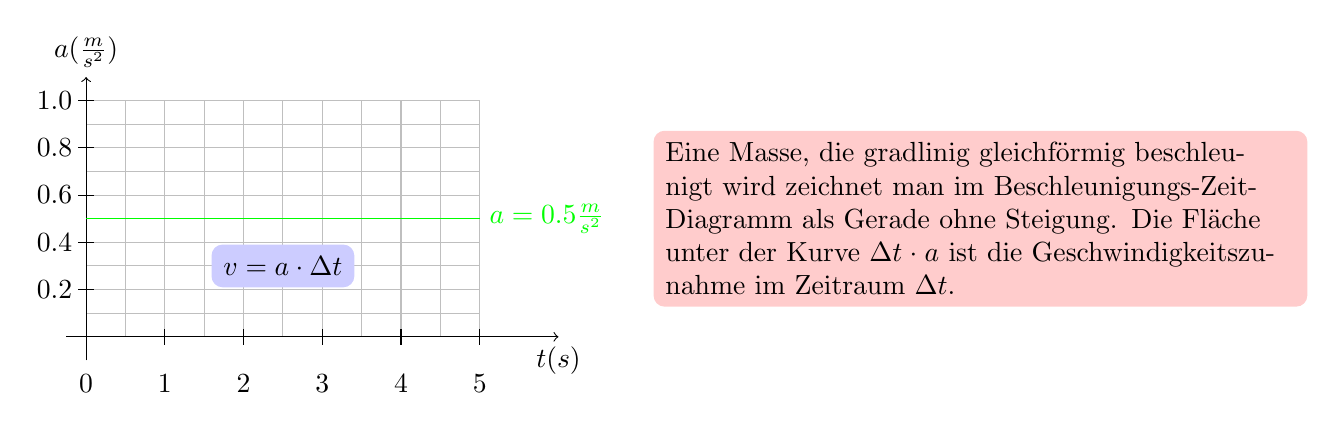
\begin{tikzpicture}[scale=1,yscale=3, info box/.style={rounded corners, inner sep=1ex}, info text/.style={info box, fill=red!20}]
\usetikzlibrary{calc,intersections,through,backgrounds}
\draw[step=0.5cm,ystep=0.1,lightgray] (0,0) grid (5.0,1.0);

%begin Koordinatensystem
%x-achse
\coordinate (C1) at (-0.25,0);
\coordinate [label=below:$t (s)$] (C2) at (6,0);
\draw  [->] (C1)--(C2);
\foreach \x in {0,1,2,3,4,5}
{
\draw (\x,-0.2) node {\x};
\draw (\x,-0.1/3)--(\x,0.1/3);
}


%y-achse
\coordinate (C3) at (0,-0.1);
\coordinate [label=above:$a (\frac{m}{s^2})$] (C4) at (0,1.1);
\draw [->] (C3)--(C4);
\foreach \y in {0.2,0.4,0.6,0.8,1.0}
{
\draw (-0.4,\y) node {\y};
\draw (-0.1,\y)--(0.1,\y);
}
%end Koordinatensystem

\draw  [color=green,domain=0:5] plot (\x,0.5) node [above,right] {$a=\SI{0.5}{\frac{m}{s^2}}$};
\draw (2.5,0.3) node [info box, fill = blue!20] {$v=a\cdot \Delta t$};

%infokasten
\draw [xshift=7.2cm] (0,0.5) node [right, text width=8cm, info text] {
Eine Masse, die  gradlinig gleichförmig beschleunigt wird zeichnet man
im Beschleunigungs-Zeit-Diagramm als Gerade ohne Steigung.
Die Fläche unter der Kurve $\Delta t\cdot a$ ist die Geschwindigkeitszunahme im Zeitraum $\Delta t$.
};



\end{tikzpicture} 


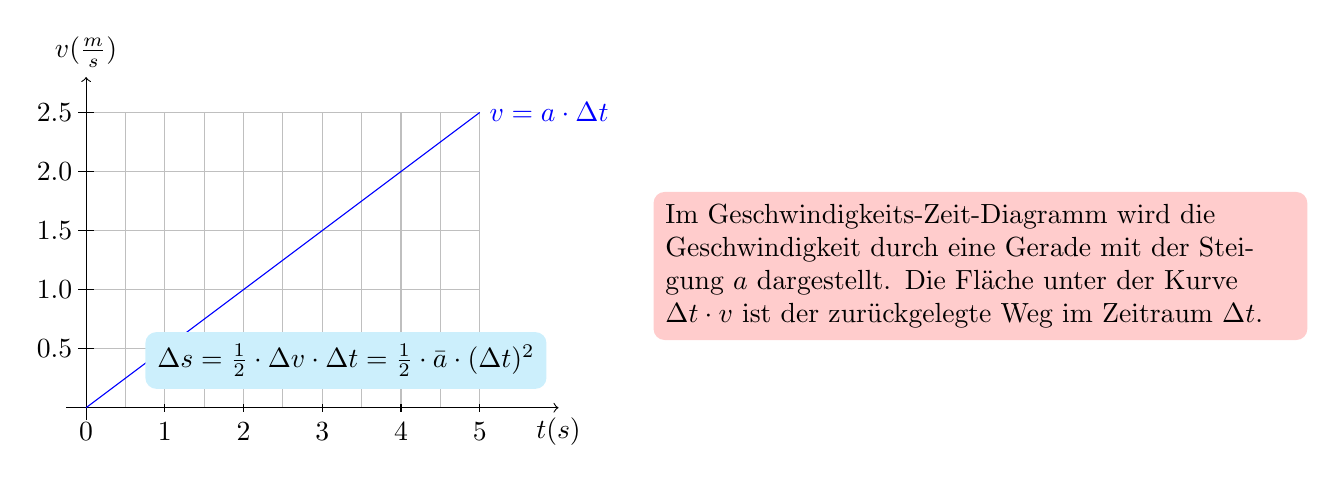
\begin{tikzpicture}[scale=1,yscale=1.5, info box/.style={rounded corners, inner sep=1ex}, info text/.style={info box, fill=red!20}]
%\usetikzlibrary{calc,intersections,through,backgrounds}
\draw[step=0.5cm,ystep=0.5,lightgray] (0,0) grid (5.0,2.5);

%begin Koordinatensystem
%x-achse
\coordinate (C1) at (-0.25,0);
\coordinate [label=below:$t (s)$] (C2) at (6,0);
\draw  [->] (C1)--(C2);
\foreach \x in {0,1,2,3,4,5}
{
\draw (\x,-0.2) node {\x};
\draw (\x,-0.1/3)--(\x,0.1/3);
}


%y-achse
\coordinate (C3) at (0,-0.1);
\coordinate [label=above:$v (\frac{m}{s})$] (C4) at (0,2.8);
\draw [->] (C3)--(C4);
\foreach \y in {0.5,1.0,1.5,2.0,2.5}
{
\draw (-0.4,\y) node {\y};
\draw (-0.1,\y)--(0.1,\y);
}
%end Koordinatensystem

\draw  [color=blue,domain=0:5] plot (\x,0.5*\x) node [above,right] {$v=a\cdot\Delta t$};
\draw (3.3,0.4) node [info box, fill =cyan!20] {$\Delta s=\frac{1}{2}\cdot \Delta v\cdot \Delta t = \frac{1}{2}\cdot\bar{a}\cdot(\Delta t)^2$};

%infokasten
\draw [xshift=7.2cm] (0,1.2) node [right, text width=8cm, info text] {
Im Geschwindigkeits-Zeit-Diagramm wird die Geschwindigkeit durch eine Gerade
mit der Steigung $a$ dargestellt. 
Die Fläche unter der Kurve $\Delta t\cdot v$ ist der zurückgelegte Weg im Zeitraum $\Delta t$.
};



\end{tikzpicture} 


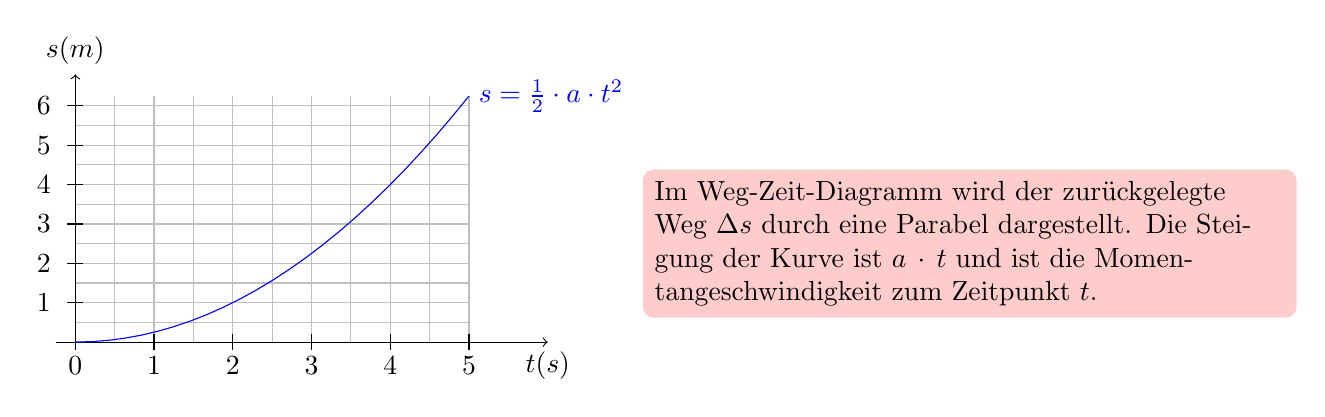
\begin{tikzpicture}[scale=1,yscale=0.5, info box/.style={rounded corners, inner sep=1ex}, info text/.style={info box, fill=red!20}]
%\usetikzlibrary{calc,intersections,through,backgrounds}
\draw[step=0.5cm,ystep=0.5,lightgray] (0,0) grid (5.0,6.25);

%begin Koordinatensystem
%x-achse
\coordinate (C1) at (-0.25,0);
\coordinate [label=below:$t (s)$] (C2) at (6,0);
\draw  [->] (C1)--(C2);
\foreach \x in {0,1,2,3,4,5}
{
\draw (\x,-0.6) node {\x};
\draw (\x,-0.1/0.5)--(\x,0.1/0.5);
}


%y-achse
\coordinate (C3) at (0,-0.1);
\coordinate [label=above:$s (m)$] (C4) at (0,6.8);
\draw [->] (C3)--(C4);
\foreach \y in {1,2,3,4,5,6}
{
\draw (-0.4,\y) node {\y};
\draw (-0.1,\y)--(0.1,\y);
}
%end Koordinatensystem

\draw  [color=blue,domain=0:5] plot (\x,0.25*\x*\x) node [above,right] {$s=\frac{1}{2}\cdot a\cdot t^2$};
%\draw (3.3,0.4) node [info box, fill =cyan!20] {$\Delta s=\frac{1}{2}\cdot \Delta v\cdot \Delta t = \frac{1}{2}\cdot\bar{a}\cdot(\Delta t)^2$};

%infokasten
\draw [xshift=7.2cm] (0,2.5) node [right, text width=8cm, info text] {
Im Weg-Zeit-Diagramm wird der zurückgelegte Weg $\Delta s$ durch eine Parabel dargestellt. 
Die Steigung der Kurve ist $a\cdot t$ und ist die Momentangeschwindigkeit zum Zeitpunkt $t$.
};



\end{tikzpicture} 




Aus den Bewegungsdiagrammen lassen sich zwei wichtige Formeln ablesen.
%\begin{cbox}
\begin{equation*}
	v=v_0+a\cdot t \qquad s=s_0 + v_0\cdot t+\frac{1}{2}\cdot a\cdot t^2
\end{equation*}
%\end{cbox}
Durch auflösen der ersten Gleichung $v=v_0+a\cdot t$ nach t und einsetzen in die zweite
bekommen wir eine Gleichung, in der die Zeit $t$ nicht vorkommt.
\begin{equation*}
	v^2=v_0^2+2\cdot a\cdot (s-s_0)
\end{equation*}

\Einbinden{\dir/beschleunigung02.tex}

%
%
%dies habe ich am SGB zum ersten und letzten mal gemacht
\section*{Der freie Fall}

Eine Masse fällt im Schwerefeld der Erde runter. Wie läuft der Fall der Masse ab?
Diese Frage kann mit dem Aufbau eines Experimentes beantwortet werden.
Dazu lassen wir eine Metallkugel aus einer vorher festgelegten Höhe zu Boden fallen.
Die Kugel benötigt für den Fall eine bestimmte Zeit $\Delta t$ die wir messen.
Um Fehler durch die Messung zu verringern, nehmen wir mehrere Zeitmessungen zu jeder
Höhenänderung vor und mitteln die Zeitspanne.
Dies wird für verschiedene Fallhöhen wiederholt. 
Die ermittelten Zeiten werden in einem Weg-Zeit-Diagramm eingetragen.


\begin{minipage}{0.5\textwidth}
%\begin{table}
	\centering
	\begin{tabular}{ccc}
		$\Delta s (\si{m})$ & $\Delta t (\si{ms})$ & $\overline{\Delta t} (\si{ms})$ \\\hline
0.1 & 129 131 130 & 130\\
0.2 & 195 200 201 & 199\\
0.3 & 241 248 244 & 244\\
0.4 & 278 285 276 & 280\\
	\end{tabular}
%	\caption{Messprotokoll für den freien Fall einer Metallkugel.}
%	\label{tab:freierfall1}
%\end{table}
\end{minipage}
\begin{minipage}{0.5\textwidth}
	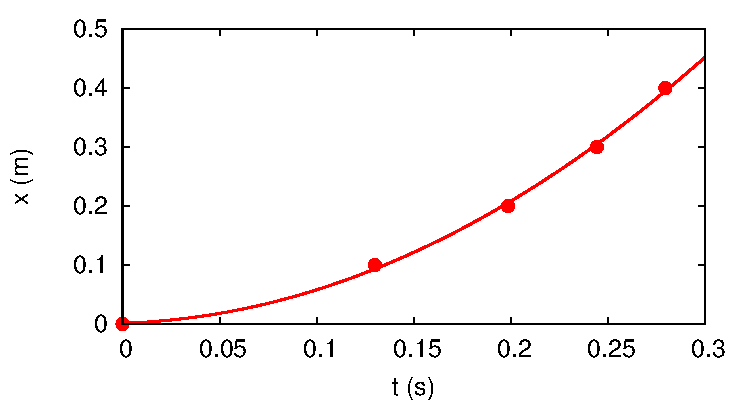
\includegraphics[width=0.95\textwidth]{./freierfall_xt.pdf}
\end{minipage}

Nun wollen wir aus dem Weg-Zeit-Diagramm ein Geschwindigkeits-Zeit-Diagramm erstellen.
Dabei gibt es einige Schwierigkeiten. Für das $v$-$t$-Diagramm wird die Momentangeschwindigkeit
benötigt. Durch die Messung kann allerdings nur eine mittlere Geschwindigkeit bestimmt werden.
Damit die mittlere Geschwindigkeit möglichst nahe an der Momentangeschwindigkeit ist, sollte eine
möglichst kleine Zeitspanne $\Delta t$ betrachtet werden.
Wir berechnen die Geschwindigkeit für die jeweils letzten \SI{10}{cm}.



\begin{minipage}{0.5\textwidth}
%\begin{table}
	\centering
	\begin{tabular}{ccc}
	$\Delta s$ &	$\Delta t (\si{s})$ & $\bar{v} (\si{m/s})$ \\\hline
%Geschwindigkeits-Zeit-Tabelle
%die letzten 10 cm
0   & 0         & 0 \\
0.1 & $\SI{130}{ms} -\SI{0}{ms}=\SI{130}{ms}$  & 0.77 \\ 
0.2 & $\SI{199}{ms} -\SI{130}{ms}=\SI{69}{ms}$  & 1.45 \\ 
0.2 & $\SI{244}{ms} -\SI{199}{ms}=\SI{45}{ms}$  & 2.22 \\ 
0.2 & $\SI{280}{ms} -\SI{244}{ms}=\SI{36}{ms}$  & 2.78 \\ 
	\end{tabular}
%	\caption{Messprotokoll für den freien Fall einer Metallkugel.}
%	\label{tab:freierfall1}
%\end{table}
\end{minipage}
\begin{minipage}{0.5\textwidth}
	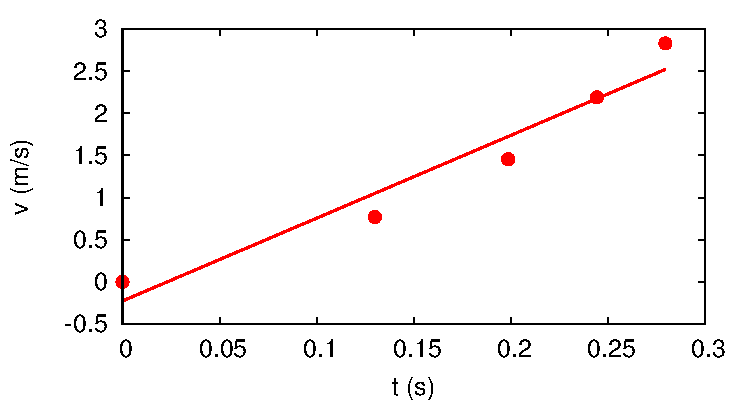
\includegraphics[width=0.95\textwidth]{./freierfall_vt.pdf}
\end{minipage}

Die berechneten Durchschnittsgeschwindigkeiten benutzen wir nun als Momentangeschwindigkeiten und tragen 
die Werte im $v$-$t$-Diagramm ein. Die Steigung der Geschwindigkeitskurve im $v$-$t$-Diagramm ist
\SI{9.92}{m/s^2}. Damit haben wir mit relativ einfachen Mitteln den Wert für die Fallbeschleunigung 
auf der Erde reproduziert und gezeigt, dass ein fallendes Objekt gleichmässig gleichförmig beschleunigt
wird, wenn es sich im Schwerefeld der Erde befindet.
Mit diesem Wissen ist es nicht mehr nötig die Momentangeschwindigkeit durch eine Durchschnittsgeschwindigkeit
zu approximieren. Stattdessen kann die Fallbeschleunigung aus dem Weg-Zeit-Diagramm bestimmt werden. 
Die Geschwindigkeit berechnet sich dann mit $v=g\cdot t$.

\section*{Bewegung in drei Raumrichtungen}

\subsection*{Vektoren}
Physikalische Grössen wie die Geschwindigkeit $v$, die Beschleunigung $a$ oder auch der Weg $s$ sind
vektorielle Grössen. Ein Vektor hat nicht nur eine Grösse, sondern auch noch eine Richtung.
Vektoren werden daher oft als Pfeile gezeichnet. Die Länge des Pfeils ist dann der Betrag des Vektors,
die Richtung des Pfeils gibt die Richtung des Vektors an.

Ein Vektor kann mit einem geeigneten Koordinatensystem in Komponenten zerlegt werden.


Vektoren kann man graphisch addieren.

%
\section*{Addition von Kräften}

In einem Knoten laufen drei Fäden zusammen. An dem jeweils anderen Ende der Fäden ist eine Masse angehängt.
Zwei der drei Fäden werden durch Rollen umgelenkt.
Wird der Knoten aus seiner Ruhelage (Gleichgewichtslage) ausgelenkt, so pendelt sich das System wieder in diese Lage zurück.
Die Rollen lenken die Fadenkräfte um, ändern aber nicht ihren Betrag.
In der Ruhelage ist die Summe aller angreifenden Kräfte Null.

\Einbinden{\dir/vektoren01.tex}
\Einbinden{\dir/vektoren02.tex}
\Einbinden{\dir/vektoren03.tex}
\Einbinden{\dir/vektoren04.tex}


\newpage
\section*{Zerlegung von Kräften}

Vektoren lassen sich nicht nur addieren, sondern man kann sie auch in Komponenten zerlegen. Das ist im Prinzip die Umkehrung
der Vektoraddition.

\Einbinden{\dir/vektoren05.tex}
\Einbinden{\dir/vektoren06.tex}


Ist die Richtung eines Vektors vorgegeben, lässt sich der Vektor noch nicht eindeutig zerlegen. Es gibt immer
noch viele verschiedene Möglichkeiten den Vektor zu zerlegen.

\newpage


Sind die Richtungen von zwei Vektoren gegeben (in 2D), ist die Zerlegung eindeutig möglich. Allgemein gilt, dass man
für jede Raumdimension eine eindeutige Richtung benötigt.

\Einbinden{\dir/vektoren07.tex}


In der Praxis zerlegt man Vektoren oft in Kartesische Koordinaten, also in eine $x$-, eine $y$- und im Fall von drei Dimensionen in eine $z$-Koordinate.

\Einbinden{\dir/vektoren08.tex}

\newpage

\Einbinden{\dir/vektoren09.tex}

\newpage
\Einbinden{\dir/vektoren10.tex}

\Einbinden{\dir/vektoren11.tex}


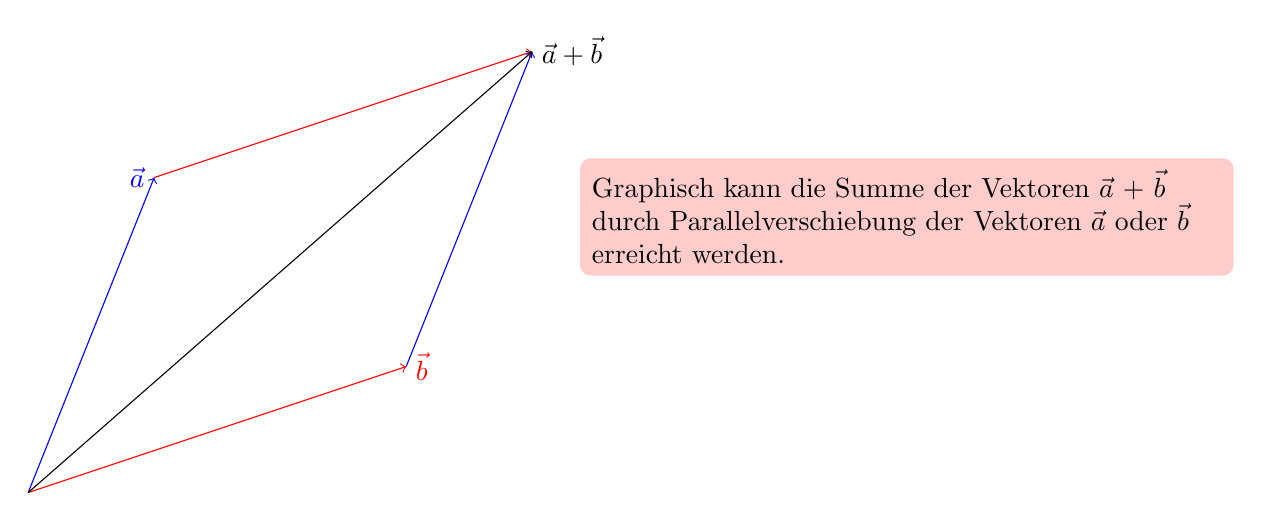
\begin{tikzpicture}[info text/.style={rounded corners, fill=red!20, inner sep=1ex}]
%\begin{tikzpicture}
%\usetikzlibrary{calc,intersections,through,backgrounds}
%\usetikzlibrary{decorations.pathmorphing}
%\draw[step=0.5cm,lightgray] (-0.5,-3.0) grid (6.5,5.0);


\draw [->, blue,scale=0.8] (0,0)--(2,5) node [left] {$\vec{a}$};
\draw[->,red,scale=0.8] (2,5)--+(6,2);

\draw[->,red,scale=0.8] (0,0)--(6,2) node [right] {$\vec{b}$};

\draw[->,blue,scale=0.8] (6,2)--+(2,5);


\draw[->,black,scale=0.8](0,0)--(8,7) node [right]{$\vec{a}+\vec{b}$};
%infokasten
\draw [xshift=7.0cm] (0,3.5) node [right, text width=8cm, info text] {
Graphisch kann die Summe der Vektoren $\vec{a}+\vec{b}$ durch Parallelverschiebung
der Vektoren $\vec{a}$ oder $\vec{b}$ erreicht werden.
};

\end{tikzpicture}

Das bedeutet, dass man eine komplizierte Bewegung, wie zum Beispiel die Bewegung eines geworfenen
Balls, oder einer Pistolenkugel für jede Raumrichtung unabhängig voneinander lösen kann.
Dies macht es erst möglich Bewegungsabläufe in mehr als einer Dimension zu berechnen.

\Einbinden{\dir/bew3d01.tex}
\Einbinden{\dir/bew3d02.tex}



%

\section*{Kräfte}
In der Physik gibt es heute vier fundamentale Kräfte. Die starke und die schwache Kernkraft, die elektromagnetische Kraft und die Gravitation.
Kräfte werden in der Physik mit dem Buchstaben $F$ abgekürzt.
Die Einheit für alle Kräfte ist das Newton N. Das Newton ist eine zusammengesetzte Einheit
\begin{eqnarray*}
	\text{N}=\frac{\text{kg}\cdot\text{m}}{\text{s}^2}\text{.}
\end{eqnarray*}

\subsection*{Gravitation}
In diesem Kapitel wollen wir uns mit der Gravitation beschäftigen. Sie wirkt auf alle Körper mit einer Masse.
Die Anziehungskraft, die ein Körper mit der Masse $m_1$ auf einen Körper mit der Masse $m_2$ ausübt, ist proportional zu den Massen $m_1$ und $m_2$.
Je grösser der Abstand zwischen den zwei Massen, desto kleiner ist die Anziehungskraft zwischen ihnen. Die Abnahme der Anziehungskraft geht quadratisch
mit dem Abstand zwischen den Körpern ein ($F\sim\nicefrac{1}{r^2}$).


\begin{aufgabe}
	Lesen Sie die obige Einführung in die Kräfte, und stellen Sie eine Gleichung für die Anziehungskraft zwischen zwei Massen her. 
\end{aufgabe}
\vspace*{2.5cm}
\begin{aufgabe}
	Welche Einheit hat die Gravitationskonstante? 
\end{aufgabe}

\vspace*{2.5cm}
%Die Gravitationskonstante G hat einen Wert von \SI{6.674E-11}{Nm^2/kg^2}
Die Gravitationskonstante G hat einen Wert von \num{6.674E-11} \gl.

\Einbinden{\dir/gravitation01.tex}
\Einbinden{\dir/gravitation02.tex}

Da es recht aufwendig ist, die Gravitationskraft zwischen Erde und den Objekten auf der Erde zu berechnen, führt man eine Vereinfachung ein.
Den Ausdruck für die Gravitationskraft formen wir um und erhalten die Gewichtskraft. 
\begin{eqnarray*}
	\RI{F}{G} = m\cdot g
\end{eqnarray*}
Der Faktor $g$ ist die Fallbeschleunigung. Es ist ein Ortsfaktor, der nicht überall auf der Erde gleich gross ist, aber immer etwa
\SI{9.81}{m/s^2} gross ist.


\Einbinden{\dir/gravitation03.tex}


\section*{Das Federgesetz}
Kräfte kann man nicht direkt beobachten. Eine Kraft muss auf einen Körper wirken, damit sie ``sichtbar'' wird.
Wirkt eine Kraft zum Beispiel auf eine Metallfeder, dann wird diese aus ihrer Ruhestellung ausgelenkt.
Wirkt die Kraft nicht mehr, nimmt die Feder wieder ihre ursprüngliche Form an. Die Verlängerung $l$ der Feder
unter Krafteinwirkung wird durch das \emph{Federgesetz} beschrieben.

\Einbinden{\dir/federgesetz01.tex}

\newcommand\leereZ{\phantom{x} & \phantom{x} & \phantom{x} \\\hline}

\subsection*{Experiment}
\begin{center}
%\begin{large}
	\begin{tabular}{p{0.3\textwidth}|p{0.3\textwidth}|p{0.3\textwidth}}
    Masse (kg) & Gewichtskraft (N) & Auslenkung (cm) \\\hline
	\leereZ
	\leereZ
	\leereZ
	\leereZ
	\leereZ
	\end{tabular}
%\end{large}
\end{center}

\begin{center}
\begin{tikzpicture}
    \mmPapier{(0,0)}{(15.5,7)}{0.5}{0.5}
\end{tikzpicture}
\end{center}

\newpage
\begin{cbox}
	\begin{center}
		\bf{Federgesetz}
	\end{center}
\begin{gather*}
	\text{Kraft} \phantom{=\text{Federkonstante}\cdot\text{Verlängerung}}\quad\text{oder}\quad F=\phantom{-D\cdot\Delta x}\\
	\text{Einheit}: [D] = \phantom{\frac{\text{Newton}}{\text{Meter}}=\frac{\si{N}}{\si{m}}}
\end{gather*}
\end{cbox}


\Einbinden{\dir/federgesetz02.tex}
\Einbinden{\dir/federgesetz03.tex}



\section*{Addition von Kräften}

In einem Knoten laufen drei Fäden zusammen. An dem jeweils anderen Ende der Fäden ist eine Masse angehängt.
Zwei der drei Fäden werden durch Rollen umgelenkt.
Wird der Knoten aus seiner Ruhelage (Gleichgewichtslage) ausgelenkt, so pendelt sich das System wieder in diese Lage zurück.
Die Rollen lenken die Fadenkräfte um, ändern aber nicht ihren Betrag.
In der Ruhelage ist die Summe aller angreifenden Kräfte Null.

\Einbinden{\dir/vektoren01.tex}
\Einbinden{\dir/vektoren02.tex}
\Einbinden{\dir/vektoren03.tex}
\Einbinden{\dir/vektoren04.tex}


\newpage
\section*{Zerlegung von Kräften}

Vektoren lassen sich nicht nur addieren, sondern man kann sie auch in Komponenten zerlegen. Das ist im Prinzip die Umkehrung
der Vektoraddition.

\Einbinden{\dir/vektoren05.tex}
\Einbinden{\dir/vektoren06.tex}


Ist die Richtung eines Vektors vorgegeben, lässt sich der Vektor noch nicht eindeutig zerlegen. Es gibt immer
noch viele verschiedene Möglichkeiten den Vektor zu zerlegen.

\newpage


Sind die Richtungen von zwei Vektoren gegeben (in 2D), ist die Zerlegung eindeutig möglich. Allgemein gilt, dass man
für jede Raumdimension eine eindeutige Richtung benötigt.

\Einbinden{\dir/vektoren07.tex}


In der Praxis zerlegt man Vektoren oft in Kartesische Koordinaten, also in eine $x$-, eine $y$- und im Fall von drei Dimensionen in eine $z$-Koordinate.

\Einbinden{\dir/vektoren08.tex}

\newpage

\Einbinden{\dir/vektoren09.tex}

\newpage
\Einbinden{\dir/vektoren10.tex}

\Einbinden{\dir/vektoren11.tex}



\section*{Das Drehmoment}
Im vorigen Abschnitt haben wir uns mit Kräften beschäftigt, die in einem Punkt eines Körpers angreifen.
Hat man es mit Kräften zu tun, die parallele verlaufen, gibt es keinen gemeinsamen Angriffspunkt mehr. 
Für diesen Fall gilt die bisherige Theorie nicht mehr.

\Einbinden{\dir/drehmomente01.tex}
\Einbinden{\dir/drehmomente02.tex}
\Einbinden{\dir/drehmomente03.tex}


\newpage
\Einbinden{\dir/drehmomente04.tex}
\Einbinden{\dir/drehmomente05.tex}


\section*{Der Schwerpunkt}

Am Schwerpunkt eines Körpers ist der Angriffspunkt der Gewichtskraft.
Lagert man einen Körper an dessen Schwerpunkt, so heben sich alle Drehmomente auf.

Den Schwerpunktes eines Punktes kann man laut Formelsammlung so berechnen:
\begin{eqnarray*}
	\vec{r}=\frac{\sum_i m_i\vec{r_i}}{\RI{m}{tot}}
\end{eqnarray*}

\Einbinden{\dir/schwerpunkt01.tex}
\Einbinden{\dir/schwerpunkt02.tex}
\Einbinden{\dir/schwerpunkt03.tex}

\newpage

\Einbinden{\dir/schwerpunkt04.tex}




\section*{Lösen von Statikproblemen mit dem Drehmoment}

%In der letzten Lektion haben wir uns mit dem Hebelgesetz beschäftigt.
%Eine bekannte Formulierung des Hebelgesetzes lautet:
%\begin{center}
%%	\begin{large}
%Kraft mal Kraftarm gleich Last mal Lastarm.
%%	\end{large}
%\end{center}

%Weiter sind wir auf das Drehmoment gestossen.
Das Drehmoment ist allgemein als Kreuzprodukt zweier Vektoren definiert:

\begin{cbox}
\begin{gather*}
	\text{Drehmoment} = \text{Kreuzprodukt von Hebelarm und Kraft} \quad\text{oder}\quad \vec{M} = \vec{r}\times\vec{F}\\
	\text{Einheit}: [\vec{M}]=\text{Meter}\cdot\text{Kraft}=\si{m}\cdot\si{N}=\si{Nm}
\end{gather*}
\end{cbox}

Das bedeutet, dass die Komponente der Kraft, die senkrecht auf dem Hebelarm steht mal dem Hebelarm gerechnet werden muss.

\Spalten{0.5}{
\Beispiel Ein realer Hebelarm hat immer auch ein Eigengewicht. Seine Gewichtskraft greift am Schwerpunkt an.
Die Richtung der Gewichtskraft ist im allgemeinen nicht senkrecht zum Hebelarm. Deshalb muss man die Gewichtskraft
zerlegen, in eine Komponente senkrecht zum Hebelarm und eine Komponente parallel zum Hebelarm.
Rechnerisch ist dass hier $\sin\alpha\cdot\RI{F}{G}$. Damit ergibt sich für das Drehmoment
\begin{eqnarray*}
	M=r\cdot \RI{F}{G}\cdot \sin\alpha\text{.}
\end{eqnarray*}
}{0.5}{
\begin{center}
	\begin{tikzpicture}

\coordinate (P0) at (30:2cm);
\draw [fill] (0,0) circle (0.1); \draw (0,0) node [left] {Drehachse};
\draw [fill] (P0) circle (0.1); \draw (P0) node [left] {Schwerpunkt};
\draw (0,0) --(30:4cm) node [ above,sloped] {Hebelarm};
\draw [Kraft,->] (P0)--++(-90:3cm) node [midway, left] {\RI{F}{G}}node [shape=coordinate] (EK){};

\draw [Winkel,->] (30:1cm) arc (210:270:1cm); \draw (P0) ++(240:0.8cm) node  {$\alpha$};

\draw [dotted] (P0)--++(-60:3cm)  node [midway,right] {$\sin\alpha\cdot\RI{F}{G}$};
\draw [dotted] (EK)--++(30:2.5cm) node [shape=coordinate] (EK){};
	\end{tikzpicture}
\end{center}
}

Zum Lösen von Problemen aus der Statik kann man das Drehmoment auch benutzen. Im statischen Fall muss die Summe der
Kräfte und die Summe der Drehmomente an jedem beliebigen Punkt Null sein.
\begin{align*}
	\vec{F_1} + \vec{F_2} + \vec{F_3} + \cdots + \vec{F_n} = 0\\
	\vec{M_1} + \vec{M_2} + \vec{M_3} + \cdots + \vec{M_n} = 0
\end{align*}


\Einbinden{\dir/loesen01.tex}
\Einbinden{\dir/loesen02.tex}



\section*{Reibung}

\Einbinden{\dir/reibung05.tex}

%\begin{table}
%	\centering
%	\begin{tabular}{ccc}
%		Materialien  & Haftreibung  & Gleitreibung \\
%		Holz auf Holz   &  \num{0.6}  & \num{0.4} \\
%		Stahl auf Stahl &  \num{0.15} & \num{0.1}\\
%		Stahl auf Eis   &  \num{0.027}& \num{0.014}\\
%	\end{tabular}
%	\caption{Haft- und Gleitreibungszahlen.}
%	\label{tab:reibung}
%\end{table}


\Einbinden{\dir/reibung06.tex}
\Einbinden{\dir/reibung07.tex}


\section*{Die schiefe Ebene}
In dieser Lektion werden wir uns mit der schiefen Ebene beschäftigen. In einem Versuch werden wir sehen, was mit einem
Klotz passiert, der auf einer angewinkelten Ebene liegt. Machen Sie sich neben den Skizzen Notizen und
zeichnen Sie alle auftretenden Kräfte ein (Gewichtskraft, Normalkraft, Reibungskraft).
Dies ist ein Beispiel, in dem Gewichtskraft und Normalkraft nicht gleich gross sind.

\subsection*{Keine Steigung der Ebene}

\Spalten{0.5}{
\begin{center}
\begin{tikzpicture}

\def\angle{0}%Winkel

\coordinate (P0) at (6,0);

\draw (0,0)--(7,0);
\draw (P0)--++(180-\angle:6);


%winkel
%\draw [->] (5,0) arc(180:180-\angle:1cm);%winkelbogen
%\draw  (P0) ++(180-0.5*\angle:0.75) node {$\alpha$};%alpha

\def\hoehe{1}
\def\breite{2}
\draw (P0) ++(180-\angle:2.25cm)--++(90-\angle:\hoehe)--++(180-\angle:\breite)--++(270-\angle:\hoehe);

%\draw [color=white] (0,-3)--(2,-3);%abstand nach unten
	\end{tikzpicture}
\end{center}
\vspace*{1.5cm}
}{0.5}{}

\subsection*{Geringe Steigung der Ebene}
\Spalten{0.5}{
\begin{center}
\begin{tikzpicture}

\def\angle{15}%Winkel

\coordinate (P0) at (6,0);

\draw (0,0)--(7,0);
\draw (P0)--++(180-\angle:6);


%winkel
\draw [->] (5,0) arc(180:180-\angle:1cm);%winkelbogen
\draw  (P0) ++(180-0.5*\angle:0.75) node {$\alpha$};%alpha

\def\hoehe{1}
\def\breite{2}
\draw (P0) ++(180-\angle:2.25cm)--++(90-\angle:\hoehe)--++(180-\angle:\breite)--++(270-\angle:\hoehe);
	\end{tikzpicture}
\end{center}
\vspace*{1.5cm}
}{0.5}{}

\subsection*{Grosse Steigung der Ebene}
\Spalten{0.5}{
\begin{center}
\begin{tikzpicture}

\def\angle{65}%Winkel

\coordinate (P0) at (6,0);

\draw (0,0)--(7,0);
\draw (P0)--++(180-\angle:6);


%winkel
\draw [->] (5,0) arc(180:180-\angle:1cm);%winkelbogen
\draw  (P0) ++(180-0.5*\angle:0.75) node {$\alpha$};%alpha

\def\hoehe{1}
\def\breite{2}
\draw (P0) ++(180-\angle:2.25cm)--++(90-\angle:\hoehe)--++(180-\angle:\breite)--++(270-\angle:\hoehe);
	\end{tikzpicture}
\end{center}
\vspace*{1.5cm}
}{0.5}{}

\Einbinden{\dir/schiefeEbene01.tex}


\section*{Die Newtonschen Axiome}

Bisher haben wir uns mit der Statik beschäftigt. In der Statik ist die Summe aller
an einen Körper angreifenden Kräfte Null. Ausserdem verschwinden alle Drehmomente bezüglich
einer beliebigen Drehachse. Ist eine dieser Bedingungen nicht erfüllt, bewegt sich der Körper.

%Bewegungen haben wir in der Kinematik untersucht.

Ausserdem haben wir die Bewegung eines Körpers durch Ort, Geschwindigkeit und Beschleunigung
beschrieben (Kinematik). Im folgenden Abschnitt wollen wir lernen \emph{warum} ein Körper sich bewegt.
Diese Gebiet der Physik wird als Dynamik bezeichnet.
Isaac Newton hat im Jahre 1686 drei Grundgesetze (Axiome) aufgestellt, die bis heute die Grundlage
der klassischen Mechanik bilden.

%Eine fundamentale Rolle in den Newtonschen Axiomen spielt die Kraft $F$.
%Die physikalische Kraft $\vec{F}$ ist eine vektorielle Grösse. Man kennt sie erst,
%wenn ihr Betrag, ihre Richtung und ihr Angriffspunkt bekannt sind. Die Einheit
%der Kraft heisst Newton.
%Eine Kraft kann man nicht direkt sehen. Wenn Gegenstände verformt werden, wie zum Beispiel
%eine Metallfeder verlängert oder gestaucht wird, dann wirken Kräfte.
%Auch wenn es zur Beschleunigung eines Gegenstands kommt sind Kräfte nötig.

Mit den folgenden Versuchen wollen wir die Newtonschen Axiome kennenlernen und
selber reproduzieren:

\subsection*{Experiment: Luftkissenbahn}

\begin{figure}[h!]
\begin{center}

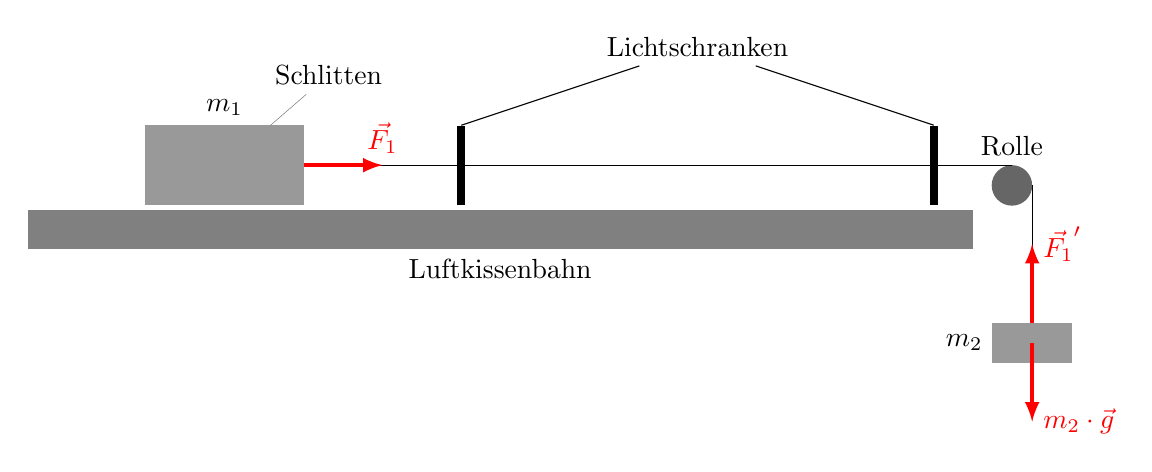
\begin{tikzpicture}
%\begin{tikzpicture}
%\usetikzlibrary{calc,intersections,through,backgrounds}
%\usetikzlibrary{decorations.pathmorphing}
%\draw[step=0.5cm,lightgray] (-0.5,-3.0) grid (6.5,5.0);
\usepgflibrary{arrows}
\tikzset{force/.style={>=latex,line width=0.05cm}}
%\newcommand{\RI}[2]{\ensuremath{#1_{\textrm{#2}}}}

\draw (5,0) node [minimum height=0.5cm, minimum width=12cm, fill, color=black!50,label=below:Luftkissenbahn] (B) {}; %bahn

\draw (B.north)+(-3.5cm,0.05cm) node [anchor=south,minimum height=1cm, minimum width=2cm,draw,fill, color=black!40, label=above:$m_1$,pin= 60:Schlitten] (M1) {}; %wagen

\draw (M1) +(10cm,0) node[anchor=north,circle,minimum size=0.5cm,draw,fill, color=black!60, label=above:Rolle] (R) {}; %rolle

\draw (R.east)+(0,-2cm) node[minimum height=0.5cm,minimum width=1cm,draw,label=left:$m_2$,fill,color=black!40] (M2) {}; %angehängtes gewicht

%\draw (M2.south)+(0,-1.2cm) node[minimum width=2cm, minimum height=0.1cm,anchor=north,fill,color=black!60, label=below:Tisch] (T){}; %Tisch

\draw (M1.east)--(R.north) (R.east)--(M2.north); %faden

%Kräfte
\draw [->,color=red,force] (M2.center)--+(-90:1cm) node [right] {$m_2\cdot \vec{g}$};
\draw[->,color=red,force] (M2.north)--+(90:1cm) node [right] {$\vec{F_1}'$};
\draw[->,color=red,force] (M1.east)--+(0:1cm) node [above]{$\vec{F_1}$};

 %Lichtschranke1}
\draw (M1.east)+(2cm,0) node[inner sep=0,minimum width=0.1cm,minimum height=1cm,fill] (L1){}; %Lichtschranke1

\draw (L1)+(6cm,0) node[inner sep=0,minimum width=0.1cm,minimum height=1cm,fill] (L2){}; %Lichtschranke1

\draw (L1.north)+(3cm,1.0cm) node (LL) {Lichtschranken};
\draw (LL)--(L1.north);
\draw (LL)--(L2.north);

\end{tikzpicture}

\end{center}
\caption{\label{fig:luftkissen} Luftkissenbahn}
\end{figure}


In folgenden wollen wir ein Experiment durchführen.
Der Versuchsaufbau ist in Abbildung~\ref{fig:luftkissen} skizziert. Ein Schlitten gleitet reibungsfrei
auf einer Luftkissenbahn. 
%Teil 1 ohne Masse m2
Im ersten Versuchsteil fehlt die Masse $m_2$. Ist der Schlitten
in Ruhe, so bleibt er an seiner Position. Hat der Schlitten eine von Null verschiedene Geschwindigkeit,
so behält er diese bei. Dies haben wir auch schon früher einmal gesehen.
Dieses Verhalten wird im ersten Newtonschen Axiom behandelt: Das Trägheitsgesetz.

\begin{cbox}
	\textbf{Das Trägheitsgesetz}\\
	``Ein Körper verharrt im Zustand der Ruhe oder der gleichförmigen Translation, sofern er nicht durch einwirkende Kräfte zur Änderung seines Zustands gezwungen wird.''\\oder im lateinischen Original:\\
	``Corpus omne perseverare in statu suo quiescendi vel movendi uniformiter in directum, nisi quatenus illud a viribus impressis cogitur statum suum mutare.''
\end{cbox}

%Teil 2 mit Masse m2
Im zweiten Versuchsaufbau verbinden wir den Schlitten mit einem Faden mit der Masse $m_2$
und untersuchen, wie sich der Bewegungszustand des Schlittens dadurch verändert.

%\newpage

\newcommand\lZIIII{\phantom{x} & \phantom{x} & \phantom{x} & \phantom{x}\\\hline}
\begin{center}
%\begin{large}
	\begin{tabular}{p{0.18\textwidth}|p{0.18\textwidth}||p{0.25\textwidth}p{0.25\textwidth}}
		\multicolumn{2}{c}{Messwerte} & \multicolumn{2}{c}{Auswertung}\\ 
    Masse $m_2$ (kg) & $\Delta t$ (s) & & \\\hline
	\lZIIII
	\lZIIII
	\lZIIII
	\lZIIII
	\lZIIII
	\lZIIII
	\lZIIII
	\lZIIII
	\end{tabular}
%\end{large}
\end{center}

\begin{aufgabe}
	\label{Fma}
	\begin{enumerate}[a)]
		\item	Beschreiben Sie den Versuch mit eigenen Worten.
		\item Werten Sie die Messwerte aus. Von Interesse sind die auf den Schlitten wirkende Kraft und die Beschleunigung des Schlittens.
		\item Tragen Sie die ausgewerteten Daten in ein Diagramm ein.
		\item Was haben Sie herausgefunden?
	\end{enumerate}
\end{aufgabe}

\newpage

\begin{cbox}\label{newton2}
	\textbf{Das Aktionsprinzip}\\
``Die Änderung der Bewegung ist der Einwirkung der bewegenden Kraft proportional und geschieht nach der Richtung derjenigen geraden Linie, nach welcher jene Kraft wirkt.''
	\\oder im lateinischen Original:\\
``Mutationem motus proportionalem esse vi motrici impressae, et fieri secundum lineam rectam qua vis illa imprimitur.''
\end{cbox}

Bekannter als diese ausformulierte Variante des zweiten Newtonschen Axioms ist die dazu gehörige Formel:
\begin{eqnarray*}
	F=m\cdot a\text{.}
\end{eqnarray*}
$F$ ist die auf einen Gegenstand wirkende Kraft, $m$ ist dessen Masse und $a$ ist die von der Kraft $F$ verursachte Beschleunigung des Körpers.
Im letzten Experiment (siehe Aufgabe \ref{Fma}) haben wir dieses Gesetz in dieser Form bestätigt.

\Einbinden{\dir/newton01.tex}
\Einbinden{\dir/newton02.tex}
\Einbinden{\dir/newton03.tex}




%für diese kapitel habe ich noch keine theorie
\section*{Kreisbewegungen}

\Einbinden{\dir/kreisbewegung_eimer.tex}
\Einbinden{\dir/kreisbewegung_reibung.tex}
\Einbinden{\dir/kreisbewegung_kanone.tex}



\begin{cbox}
	\textbf{Das Wechselwirkungsgesetz}\\
	``Kräfte treten immer paarweise auf. Übt ein Körper A auf einen anderen Körper B eine Kraft aus (actio), so wirkt eine gleich große, aber entgegen gerichtete Kraft von Körper B auf Körper A (reactio).''\\oder im lateinischen Original:\\
	``Actioni contrariam semper et aequalem esse reactionem: sive corporum duorum actiones in se mutuo semper esse aequales et in partes contrarias dirigi.''
\end{cbox}

\Einbinden{\dir/wechselwirkung01.tex}
\Einbinden{\dir/wechselwirkung02.tex}

\section*{Der Impuls}
Der Impuls $\vec{p}$ eines Teilchens ist definiert als das Produkt aus seiner Masse und seiner Geschwindigkeit:
\begin{cbox}
\begin{gather*}
	\text{Impuls} = \text{Produkt von Masse und Geschwindigkeit} \quad\text{oder}\quad \vec{p} = m\cdot\vec{v}\\
	\text{Einheit}: [\vec{p}]=\text{Kilogramm}\cdot\nicefrac{\text{Meter}}{\text{Sekunde}}=\si{kg}\cdot\si{m/s}=\si{N s}
\end{gather*}
\end{cbox}

\Einbinden{\dir/impuls01.tex}

Wirken keine äusseren Kräfte auf ein System, so bleibt der  Gesamtimpuls erhalten. 
Schauen Sie sich dazu noch einmal Aufgabe \ref{skateboard} an.
Nehmen wir an, der Ball habe eine Masse von \SI{2}{kg}, Mensch und Skateboard zusammen wiegen \SI{50}{kg}.
Reibung soll vernachlässigt werden.
Der Gesamtimpuls vor dem Werfen ist Null, da das Skateboard in Ruhe ist.
Nun wird der Ball beschleunigt und erhält eine Geschwindigkeit von \SI{10}{m/s}.
Der Impuls des Balls ist damit
\begin{eqnarray*}
	p=m\cdot v=\SI{2}{kg}\cdot\SI{10}{m/s}=\SI{20}{kg m/s}\text{.}
\end{eqnarray*}
Da der Gesamtimpuls Null bleibt, rollt das Skateboard mit Fahrer in die entgegengesetzte Richtung weg.
Die Geschwindigkeit ist: 
\begin{eqnarray*}
	p=m\cdot v\to v=\frac{p}{m}=\frac{\SI{20}{kg m/s}}{\SI{50}{kg}}=\SI{0.4}{m/s}\text{.}
\end{eqnarray*}

\section*{Arbeit und Energie}
In der Umgangssprache ist der Begriff \emph{Arbeit} nicht klar definiert.
Viele Menschen arbeiten im Büro und schreiben, telefonieren und diskutieren.
Andere arbeiten auf Baustellen und tragen Steine und schweres Gerät.

In der Physik ist die \emph{Arbeit} klar definiert.
\emph{Arbeit} ist das Skalarprodukt aus \emph{Kraft} und \emph{Weg}.
Die Einheit der Arbeit ist das {\bf Joule}.

\begin{cbox}
\begin{gather*}
    \text{Arbeit} = \text{Kraft}\cdot{\text{Weg}}\quad\text{oder}\quad W=F\cdot s\cdot \cos \alpha\\
	\text{Einheit}: [W] = \text{Newton}\cdot\text{Meter}=\si{N}\cdot\si{m}=\frac{\si{kg}\cdot\si{m}}{\si{s^2}}\cdot \si{m}=\text{Joule}=\si{J}
\end{gather*}
\end{cbox}

\Einbinden{\dir/arbeit_schrank.tex}
\Einbinden{\dir/arbeit_schlitten.tex}


\subsection*{Hubarbeit}
Um einen Körper der Masse $m$ um eine Höhe $h$ anzuheben, ist eine \emph{Hubarbeit} erforderlich.
\begin{equation*}
	W_{\text{Hub}} = F \cdot h = F_{\text{G}}\cdot h = m\cdot g\cdot h
\end{equation*}

Im Vergleich zu seiner ursprünglichen Lage hat der Körper eine höhere potentielle Energie.

\begin{cbox}
\begin{equation*}
	E_{\text{pot}} = m\cdot g\cdot h
\end{equation*}
\end{cbox}


\Einbinden{\dir/arbeit_hub.tex}




\subsection*{Beschleunigungsarbeit}
Um einen Körper zu beschleunigen ist eine Kraft nötig. Es gilt $F=m\cdot a$ wie wir auf Seite ~\pageref{newton2} gesehen haben.
Damit ist klar, dass es auch eine Beschleunigungsarbeit gibt.
\begin{eqnarray*}
	\RI{W}{Bew}=F\cdot s=m\cdot a\cdot s=\frac{1}{2}\cdot m\cdot\left(v^2-v_0^2\right)
\end{eqnarray*}

Dabei ist $m$ die Masse, $a$ die Beschleunigung, $s$ der Weg und $v$ die Geschwindigkeit.
Im letzten Schritt haben wir für $a\cdot s$ einen Ausdruck eingesetzt, den wir durch umstellen aus der Formel
$v^2=v_0^2+2\cdot a\cdot s$ bekommen haben.

Hat der Körper die Geschwindigkeit $v$ erreicht, so besitzt er eine \emph{kinetische Energie}.

\begin{cbox}
\begin{equation*}
	\RI{E}{kin} = \frac{1}{2}\cdot m\cdot v^2
\end{equation*}
\end{cbox}

\Einbinden{\dir/arbeit_velo.tex}
\Einbinden{\dir/Ekin_auto.tex}

\newpage

\subsection*{Verformungsarbeit}
In diesem Abschnitt werden wir lernen, wie man die Arbeit für eine nicht konstante Kraft bestimmen kann.
Arbeit ist Kraft mal Weg. Ändert sich die Kraft über den Weg, muss man dies berücksichtigen.

\begin{figure}[h!]
\begin{center}
\begin{tikzpicture}[gnuplot]
%% generated with GNUPLOT 4.6p1 (Lua 5.1; terminal rev. 99, script rev. 100)
%% Mit 05 Dez 2012 16:08:51 CET
\path (0.000,0.000) rectangle (15.000,5.000);
\gpcolor{color=gp lt color border}
\gpsetlinetype{gp lt border}
\gpsetlinewidth{1.00}
\draw[gp path] (1.320,4.631)--(1.320,0.985)--(6.947,0.985)--(6.947,4.631)--cycle;
\node[gp node center,rotate=-270] at (0.246,2.808) {Kraft (N)};
\node[gp node center] at (4.133,0.215) {Weg (m)};
\gpfill{rgb color={0.063,0.318,0.502}} (1.320,0.985)--(1.320,0.985)--(1.377,1.022)--(1.434,1.059)%
    --(1.491,1.095)--(1.547,1.132)--(1.604,1.169)--(1.661,1.206)--(1.718,1.243)%
    --(1.775,1.280)--(1.832,1.316)--(1.888,1.353)--(1.945,1.390)--(2.002,1.427)%
    --(2.059,1.464)--(2.116,1.501)--(2.173,1.537)--(2.229,1.574)--(2.286,1.611)%
    --(2.343,1.648)--(2.400,1.685)--(2.457,1.722)--(2.514,1.758)--(2.570,1.795)%
    --(2.627,1.832)--(2.684,1.869)--(2.741,1.906)--(2.798,1.943)--(2.855,1.979)%
    --(2.911,2.016)--(2.968,2.053)--(3.025,2.090)--(3.082,2.127)--(3.139,2.164)%
    --(3.196,2.200)--(3.253,2.237)--(3.309,2.274)--(3.366,2.311)--(3.423,2.348)%
    --(3.480,2.384)--(3.537,2.421)--(3.594,2.458)--(3.650,2.495)--(3.707,2.532)%
    --(3.764,2.569)--(3.821,2.605)--(3.878,2.642)--(3.935,2.679)--(3.991,2.716)%
    --(4.048,2.753)--(4.105,2.790)--(4.162,2.826)--(4.219,2.863)--(4.276,2.900)%
    --(4.332,2.937)--(4.389,2.974)--(4.446,3.011)--(4.503,3.047)--(4.560,3.084)%
    --(4.617,3.121)--(4.673,3.158)--(4.730,3.195)--(4.787,3.232)--(4.844,3.268)%
    --(4.901,3.305)--(4.958,3.342)--(5.014,3.379)--(5.071,3.416)--(5.128,3.452)%
    --(5.185,3.489)--(5.242,3.526)--(5.299,3.563)--(5.356,3.600)--(5.412,3.637)%
    --(5.469,3.673)--(5.526,3.710)--(5.583,3.747)--(5.640,3.784)--(5.697,3.821)%
    --(5.753,3.858)--(5.810,3.894)--(5.867,3.931)--(5.924,3.968)--(5.981,4.005)%
    --(6.038,4.042)--(6.094,4.079)--(6.151,4.115)--(6.208,4.152)--(6.265,4.189)%
    --(6.322,4.226)--(6.379,4.263)--(6.435,4.300)--(6.492,4.336)--(6.549,4.373)%
    --(6.606,4.410)--(6.663,4.447)--(6.720,4.484)--(6.776,4.521)--(6.833,4.557)%
    --(6.890,4.594)--(6.947,4.631)--(6.947,0.985)--cycle;
\gpcolor{rgb color={0.063,0.318,0.502}}
\gpsetlinetype{gp lt plot 0}
\gpsetlinewidth{4.00}
\draw[gp path] (1.320,0.985)--(1.377,1.022)--(1.434,1.059)--(1.491,1.095)--(1.547,1.132)%
  --(1.604,1.169)--(1.661,1.206)--(1.718,1.243)--(1.775,1.280)--(1.832,1.316)--(1.888,1.353)%
  --(1.945,1.390)--(2.002,1.427)--(2.059,1.464)--(2.116,1.501)--(2.173,1.537)--(2.229,1.574)%
  --(2.286,1.611)--(2.343,1.648)--(2.400,1.685)--(2.457,1.722)--(2.514,1.758)--(2.570,1.795)%
  --(2.627,1.832)--(2.684,1.869)--(2.741,1.906)--(2.798,1.943)--(2.855,1.979)--(2.911,2.016)%
  --(2.968,2.053)--(3.025,2.090)--(3.082,2.127)--(3.139,2.164)--(3.196,2.200)--(3.253,2.237)%
  --(3.309,2.274)--(3.366,2.311)--(3.423,2.348)--(3.480,2.384)--(3.537,2.421)--(3.594,2.458)%
  --(3.650,2.495)--(3.707,2.532)--(3.764,2.569)--(3.821,2.605)--(3.878,2.642)--(3.935,2.679)%
  --(3.991,2.716)--(4.048,2.753)--(4.105,2.790)--(4.162,2.826)--(4.219,2.863)--(4.276,2.900)%
  --(4.332,2.937)--(4.389,2.974)--(4.446,3.011)--(4.503,3.047)--(4.560,3.084)--(4.617,3.121)%
  --(4.673,3.158)--(4.730,3.195)--(4.787,3.232)--(4.844,3.268)--(4.901,3.305)--(4.958,3.342)%
  --(5.014,3.379)--(5.071,3.416)--(5.128,3.452)--(5.185,3.489)--(5.242,3.526)--(5.299,3.563)%
  --(5.356,3.600)--(5.412,3.637)--(5.469,3.673)--(5.526,3.710)--(5.583,3.747)--(5.640,3.784)%
  --(5.697,3.821)--(5.753,3.858)--(5.810,3.894)--(5.867,3.931)--(5.924,3.968)--(5.981,4.005)%
  --(6.038,4.042)--(6.094,4.079)--(6.151,4.115)--(6.208,4.152)--(6.265,4.189)--(6.322,4.226)%
  --(6.379,4.263)--(6.435,4.300)--(6.492,4.336)--(6.549,4.373)--(6.606,4.410)--(6.663,4.447)%
  --(6.720,4.484)--(6.776,4.521)--(6.833,4.557)--(6.890,4.594)--(6.947,4.631);
\gpcolor{color=gp lt color axes}
\gpsetlinetype{gp lt axes}
\gpsetlinewidth{1.00}
\draw[gp path] (1.320,0.985)--(6.947,0.985);
\gpcolor{color=gp lt color border}
\gpsetlinetype{gp lt border}
\draw[gp path] (1.320,0.985)--(1.500,0.985);
\draw[gp path] (6.947,0.985)--(6.767,0.985);
\node[gp node right] at (1.136,0.985) { 0};
\gpcolor{color=gp lt color axes}
\gpsetlinetype{gp lt axes}
\draw[gp path] (1.320,1.593)--(6.947,1.593);
\gpcolor{color=gp lt color border}
\gpsetlinetype{gp lt border}
\draw[gp path] (1.320,1.593)--(1.500,1.593);
\draw[gp path] (6.947,1.593)--(6.767,1.593);
\node[gp node right] at (1.136,1.593) { 5};
\gpcolor{color=gp lt color axes}
\gpsetlinetype{gp lt axes}
\draw[gp path] (1.320,2.200)--(6.947,2.200);
\gpcolor{color=gp lt color border}
\gpsetlinetype{gp lt border}
\draw[gp path] (1.320,2.200)--(1.500,2.200);
\draw[gp path] (6.947,2.200)--(6.767,2.200);
\node[gp node right] at (1.136,2.200) { 10};
\gpcolor{color=gp lt color axes}
\gpsetlinetype{gp lt axes}
\draw[gp path] (1.320,2.808)--(6.947,2.808);
\gpcolor{color=gp lt color border}
\gpsetlinetype{gp lt border}
\draw[gp path] (1.320,2.808)--(1.500,2.808);
\draw[gp path] (6.947,2.808)--(6.767,2.808);
\node[gp node right] at (1.136,2.808) { 15};
\gpcolor{color=gp lt color axes}
\gpsetlinetype{gp lt axes}
\draw[gp path] (1.320,3.416)--(6.947,3.416);
\gpcolor{color=gp lt color border}
\gpsetlinetype{gp lt border}
\draw[gp path] (1.320,3.416)--(1.500,3.416);
\draw[gp path] (6.947,3.416)--(6.767,3.416);
\node[gp node right] at (1.136,3.416) { 20};
\gpcolor{color=gp lt color axes}
\gpsetlinetype{gp lt axes}
\draw[gp path] (1.320,4.023)--(6.947,4.023);
\gpcolor{color=gp lt color border}
\gpsetlinetype{gp lt border}
\draw[gp path] (1.320,4.023)--(1.500,4.023);
\draw[gp path] (6.947,4.023)--(6.767,4.023);
\node[gp node right] at (1.136,4.023) { 25};
\gpcolor{color=gp lt color axes}
\gpsetlinetype{gp lt axes}
\draw[gp path] (1.320,4.631)--(6.947,4.631);
\gpcolor{color=gp lt color border}
\gpsetlinetype{gp lt border}
\draw[gp path] (1.320,4.631)--(1.500,4.631);
\draw[gp path] (6.947,4.631)--(6.767,4.631);
\node[gp node right] at (1.136,4.631) { 30};
\gpcolor{color=gp lt color axes}
\gpsetlinetype{gp lt axes}
\draw[gp path] (1.320,0.985)--(1.320,4.631);
\gpcolor{color=gp lt color border}
\gpsetlinetype{gp lt border}
\draw[gp path] (1.320,0.985)--(1.320,1.165);
\draw[gp path] (1.320,4.631)--(1.320,4.451);
\node[gp node center] at (1.320,0.677) { 0};
\gpcolor{color=gp lt color axes}
\gpsetlinetype{gp lt axes}
\draw[gp path] (2.445,0.985)--(2.445,4.631);
\gpcolor{color=gp lt color border}
\gpsetlinetype{gp lt border}
\draw[gp path] (2.445,0.985)--(2.445,1.165);
\draw[gp path] (2.445,4.631)--(2.445,4.451);
\node[gp node center] at (2.445,0.677) { 0.05};
\gpcolor{color=gp lt color axes}
\gpsetlinetype{gp lt axes}
\draw[gp path] (3.571,0.985)--(3.571,4.631);
\gpcolor{color=gp lt color border}
\gpsetlinetype{gp lt border}
\draw[gp path] (3.571,0.985)--(3.571,1.165);
\draw[gp path] (3.571,4.631)--(3.571,4.451);
\node[gp node center] at (3.571,0.677) { 0.1};
\gpcolor{color=gp lt color axes}
\gpsetlinetype{gp lt axes}
\draw[gp path] (4.696,0.985)--(4.696,4.631);
\gpcolor{color=gp lt color border}
\gpsetlinetype{gp lt border}
\draw[gp path] (4.696,0.985)--(4.696,1.165);
\draw[gp path] (4.696,4.631)--(4.696,4.451);
\node[gp node center] at (4.696,0.677) { 0.15};
\gpcolor{color=gp lt color axes}
\gpsetlinetype{gp lt axes}
\draw[gp path] (5.822,0.985)--(5.822,4.451)--(5.822,4.631);
\gpcolor{color=gp lt color border}
\gpsetlinetype{gp lt border}
\draw[gp path] (5.822,0.985)--(5.822,1.165);
\draw[gp path] (5.822,4.631)--(5.822,4.451);
\node[gp node center] at (5.822,0.677) { 0.2};
\gpcolor{color=gp lt color axes}
\gpsetlinetype{gp lt axes}
\draw[gp path] (6.947,0.985)--(6.947,4.631);
\gpcolor{color=gp lt color border}
\gpsetlinetype{gp lt border}
\draw[gp path] (6.947,0.985)--(6.947,1.165);
\draw[gp path] (6.947,4.631)--(6.947,4.451);
\node[gp node center] at (6.947,0.677) { 0.25};
\draw[gp path] (1.320,4.631)--(1.320,0.985)--(6.947,0.985)--(6.947,4.631)--cycle;
%% coordinates of the plot area
\gpdefrectangularnode{gp plot 1}{\pgfpoint{1.320cm}{0.985cm}}{\pgfpoint{6.947cm}{4.631cm}}
\draw[gp path] (9.004,4.631)--(9.004,0.985)--(14.447,0.985)--(14.447,4.631)--cycle;
\node[gp node center,rotate=-270] at (7.746,2.808) {Kraft (N)};
\node[gp node center] at (11.725,0.215) {Weg (m)};
\gpfill{rgb color={0.063,0.318,0.502}} (9.004,0.985)--(9.004,0.985)--(9.059,1.048)--(9.114,1.111)%
    --(9.169,1.174)--(9.224,1.237)--(9.279,1.300)--(9.334,1.363)--(9.389,1.425)%
    --(9.444,1.488)--(9.499,1.550)--(9.554,1.612)--(9.609,1.673)--(9.664,1.734)%
    --(9.719,1.795)--(9.774,1.856)--(9.829,1.916)--(9.884,1.976)--(9.939,2.035)%
    --(9.994,2.094)--(10.049,2.152)--(10.104,2.210)--(10.159,2.267)--(10.214,2.324)%
    --(10.269,2.380)--(10.324,2.435)--(10.378,2.490)--(10.433,2.544)--(10.488,2.598)%
    --(10.543,2.650)--(10.598,2.703)--(10.653,2.754)--(10.708,2.804)--(10.763,2.854)%
    --(10.818,2.903)--(10.873,2.952)--(10.928,2.999)--(10.983,3.045)--(11.038,3.091)%
    --(11.093,3.136)--(11.148,3.180)--(11.203,3.223)--(11.258,3.265)--(11.313,3.307)%
    --(11.368,3.347)--(11.423,3.386)--(11.478,3.425)--(11.533,3.463)--(11.588,3.499)%
    --(11.643,3.535)--(11.698,3.570)--(11.753,3.603)--(11.808,3.636)--(11.863,3.668)%
    --(11.918,3.699)--(11.973,3.729)--(12.028,3.758)--(12.083,3.786)--(12.138,3.813)%
    --(12.193,3.839)--(12.248,3.865)--(12.303,3.889)--(12.358,3.912)--(12.413,3.935)%
    --(12.468,3.956)--(12.523,3.977)--(12.578,3.997)--(12.633,4.016)--(12.688,4.034)%
    --(12.743,4.051)--(12.798,4.067)--(12.853,4.083)--(12.908,4.097)--(12.963,4.111)%
    --(13.018,4.124)--(13.073,4.136)--(13.127,4.148)--(13.182,4.159)--(13.237,4.169)%
    --(13.292,4.178)--(13.347,4.187)--(13.402,4.195)--(13.457,4.203)--(13.512,4.210)%
    --(13.567,4.216)--(13.622,4.222)--(13.677,4.227)--(13.732,4.231)--(13.787,4.236)%
    --(13.842,4.239)--(13.897,4.243)--(13.952,4.245)--(14.007,4.248)--(14.062,4.250)%
    --(14.117,4.252)--(14.172,4.253)--(14.227,4.255)--(14.282,4.255)--(14.337,4.256)%
    --(14.392,4.257)--(14.447,4.257)--(14.447,0.985)--cycle;
\gpcolor{rgb color={0.063,0.318,0.502}}
\gpsetlinetype{gp lt plot 0}
\gpsetlinewidth{4.00}
\draw[gp path] (9.004,0.985)--(9.059,1.048)--(9.114,1.111)--(9.169,1.174)--(9.224,1.237)%
  --(9.279,1.300)--(9.334,1.363)--(9.389,1.425)--(9.444,1.488)--(9.499,1.550)--(9.554,1.612)%
  --(9.609,1.673)--(9.664,1.734)--(9.719,1.795)--(9.774,1.856)--(9.829,1.916)--(9.884,1.976)%
  --(9.939,2.035)--(9.994,2.094)--(10.049,2.152)--(10.104,2.210)--(10.159,2.267)--(10.214,2.324)%
  --(10.269,2.380)--(10.324,2.435)--(10.378,2.490)--(10.433,2.544)--(10.488,2.598)--(10.543,2.650)%
  --(10.598,2.703)--(10.653,2.754)--(10.708,2.804)--(10.763,2.854)--(10.818,2.903)--(10.873,2.952)%
  --(10.928,2.999)--(10.983,3.045)--(11.038,3.091)--(11.093,3.136)--(11.148,3.180)--(11.203,3.223)%
  --(11.258,3.265)--(11.313,3.307)--(11.368,3.347)--(11.423,3.386)--(11.478,3.425)--(11.533,3.463)%
  --(11.588,3.499)--(11.643,3.535)--(11.698,3.570)--(11.753,3.603)--(11.808,3.636)--(11.863,3.668)%
  --(11.918,3.699)--(11.973,3.729)--(12.028,3.758)--(12.083,3.786)--(12.138,3.813)--(12.193,3.839)%
  --(12.248,3.865)--(12.303,3.889)--(12.358,3.912)--(12.413,3.935)--(12.468,3.956)--(12.523,3.977)%
  --(12.578,3.997)--(12.633,4.016)--(12.688,4.034)--(12.743,4.051)--(12.798,4.067)--(12.853,4.083)%
  --(12.908,4.097)--(12.963,4.111)--(13.018,4.124)--(13.073,4.136)--(13.127,4.148)--(13.182,4.159)%
  --(13.237,4.169)--(13.292,4.178)--(13.347,4.187)--(13.402,4.195)--(13.457,4.203)--(13.512,4.210)%
  --(13.567,4.216)--(13.622,4.222)--(13.677,4.227)--(13.732,4.231)--(13.787,4.236)--(13.842,4.239)%
  --(13.897,4.243)--(13.952,4.245)--(14.007,4.248)--(14.062,4.250)--(14.117,4.252)--(14.172,4.253)%
  --(14.227,4.255)--(14.282,4.255)--(14.337,4.256)--(14.392,4.257)--(14.447,4.257);
\gpcolor{color=gp lt color axes}
\gpsetlinetype{gp lt axes}
\gpsetlinewidth{1.00}
\draw[gp path] (9.004,0.985)--(14.447,0.985);
\gpcolor{color=gp lt color border}
\gpsetlinetype{gp lt border}
\draw[gp path] (9.004,0.985)--(9.184,0.985);
\draw[gp path] (14.447,0.985)--(14.267,0.985);
\node[gp node right] at (8.820,0.985) { 0};
\gpcolor{color=gp lt color axes}
\gpsetlinetype{gp lt axes}
\draw[gp path] (9.004,1.506)--(14.447,1.506);
\gpcolor{color=gp lt color border}
\gpsetlinetype{gp lt border}
\draw[gp path] (9.004,1.506)--(9.184,1.506);
\draw[gp path] (14.447,1.506)--(14.267,1.506);
\node[gp node right] at (8.820,1.506) { 0.5};
\gpcolor{color=gp lt color axes}
\gpsetlinetype{gp lt axes}
\draw[gp path] (9.004,2.027)--(14.447,2.027);
\gpcolor{color=gp lt color border}
\gpsetlinetype{gp lt border}
\draw[gp path] (9.004,2.027)--(9.184,2.027);
\draw[gp path] (14.447,2.027)--(14.267,2.027);
\node[gp node right] at (8.820,2.027) { 1};
\gpcolor{color=gp lt color axes}
\gpsetlinetype{gp lt axes}
\draw[gp path] (9.004,2.548)--(14.447,2.548);
\gpcolor{color=gp lt color border}
\gpsetlinetype{gp lt border}
\draw[gp path] (9.004,2.548)--(9.184,2.548);
\draw[gp path] (14.447,2.548)--(14.267,2.548);
\node[gp node right] at (8.820,2.548) { 1.5};
\gpcolor{color=gp lt color axes}
\gpsetlinetype{gp lt axes}
\draw[gp path] (9.004,3.068)--(14.447,3.068);
\gpcolor{color=gp lt color border}
\gpsetlinetype{gp lt border}
\draw[gp path] (9.004,3.068)--(9.184,3.068);
\draw[gp path] (14.447,3.068)--(14.267,3.068);
\node[gp node right] at (8.820,3.068) { 2};
\gpcolor{color=gp lt color axes}
\gpsetlinetype{gp lt axes}
\draw[gp path] (9.004,3.589)--(14.447,3.589);
\gpcolor{color=gp lt color border}
\gpsetlinetype{gp lt border}
\draw[gp path] (9.004,3.589)--(9.184,3.589);
\draw[gp path] (14.447,3.589)--(14.267,3.589);
\node[gp node right] at (8.820,3.589) { 2.5};
\gpcolor{color=gp lt color axes}
\gpsetlinetype{gp lt axes}
\draw[gp path] (9.004,4.110)--(14.447,4.110);
\gpcolor{color=gp lt color border}
\gpsetlinetype{gp lt border}
\draw[gp path] (9.004,4.110)--(9.184,4.110);
\draw[gp path] (14.447,4.110)--(14.267,4.110);
\node[gp node right] at (8.820,4.110) { 3};
\gpcolor{color=gp lt color axes}
\gpsetlinetype{gp lt axes}
\draw[gp path] (9.004,4.631)--(14.447,4.631);
\gpcolor{color=gp lt color border}
\gpsetlinetype{gp lt border}
\draw[gp path] (9.004,4.631)--(9.184,4.631);
\draw[gp path] (14.447,4.631)--(14.267,4.631);
\node[gp node right] at (8.820,4.631) { 3.5};
\gpcolor{color=gp lt color axes}
\gpsetlinetype{gp lt axes}
\draw[gp path] (9.004,0.985)--(9.004,4.631);
\gpcolor{color=gp lt color border}
\gpsetlinetype{gp lt border}
\draw[gp path] (9.004,0.985)--(9.004,1.165);
\draw[gp path] (9.004,4.631)--(9.004,4.451);
\node[gp node center] at (9.004,0.677) { 0};
\gpcolor{color=gp lt color axes}
\gpsetlinetype{gp lt axes}
\draw[gp path] (9.911,0.985)--(9.911,4.631);
\gpcolor{color=gp lt color border}
\gpsetlinetype{gp lt border}
\draw[gp path] (9.911,0.985)--(9.911,1.165);
\draw[gp path] (9.911,4.631)--(9.911,4.451);
\node[gp node center] at (9.911,0.677) { 0.5};
\gpcolor{color=gp lt color axes}
\gpsetlinetype{gp lt axes}
\draw[gp path] (10.818,0.985)--(10.818,4.631);
\gpcolor{color=gp lt color border}
\gpsetlinetype{gp lt border}
\draw[gp path] (10.818,0.985)--(10.818,1.165);
\draw[gp path] (10.818,4.631)--(10.818,4.451);
\node[gp node center] at (10.818,0.677) { 1};
\gpcolor{color=gp lt color axes}
\gpsetlinetype{gp lt axes}
\draw[gp path] (11.726,0.985)--(11.726,4.631);
\gpcolor{color=gp lt color border}
\gpsetlinetype{gp lt border}
\draw[gp path] (11.726,0.985)--(11.726,1.165);
\draw[gp path] (11.726,4.631)--(11.726,4.451);
\node[gp node center] at (11.726,0.677) { 1.5};
\gpcolor{color=gp lt color axes}
\gpsetlinetype{gp lt axes}
\draw[gp path] (12.633,0.985)--(12.633,4.631);
\gpcolor{color=gp lt color border}
\gpsetlinetype{gp lt border}
\draw[gp path] (12.633,0.985)--(12.633,1.165);
\draw[gp path] (12.633,4.631)--(12.633,4.451);
\node[gp node center] at (12.633,0.677) { 2};
\gpcolor{color=gp lt color axes}
\gpsetlinetype{gp lt axes}
\draw[gp path] (13.540,0.985)--(13.540,4.451)--(13.540,4.631);
\gpcolor{color=gp lt color border}
\gpsetlinetype{gp lt border}
\draw[gp path] (13.540,0.985)--(13.540,1.165);
\draw[gp path] (13.540,4.631)--(13.540,4.451);
\node[gp node center] at (13.540,0.677) { 2.5};
\gpcolor{color=gp lt color axes}
\gpsetlinetype{gp lt axes}
\draw[gp path] (14.447,0.985)--(14.447,4.631);
\gpcolor{color=gp lt color border}
\gpsetlinetype{gp lt border}
\draw[gp path] (14.447,0.985)--(14.447,1.165);
\draw[gp path] (14.447,4.631)--(14.447,4.451);
\node[gp node center] at (14.447,0.677) { 3};
\draw[gp path] (9.004,4.631)--(9.004,0.985)--(14.447,0.985)--(14.447,4.631)--cycle;
%% coordinates of the plot area
\gpdefrectangularnode{gp plot 2}{\pgfpoint{9.004cm}{0.985cm}}{\pgfpoint{14.447cm}{4.631cm}}
\end{tikzpicture}
%% gnuplot variables

\end{center}
\caption{\label{fig:arbeitsdiagramm} Arbeitsdiagramm für eine ideale Feder und für eine reale Feder.
}
\end{figure}

In Abbildung~\ref{fig:arbeitsdiagramm} sehen wir zwei verschiedene Arbeitsdiagramme. 
Das erste Arbeitsdiagramm zeigt die Arbeit zum spannen einer idealen Feder.
Die Federkraft ist ein Beispiel für eine nicht konstante Kraft. 
%Wie wir schon auf Seite \pageref{hook} gesehen haben, 
Wie wir schon früher einmal gesehen haben,
gilt für die Federkraft $\RI{F}{F} = -D\cdot l$. Dabei ist $D$ die Federkonstante
und $l$ ist die Auslenkung aus der Ruhelage der Feder.
Die Federkraft nimmt linear mit der Auslenkung der Feder zu. Das heisst, am Anfang ist relativ wenig
Arbeit nötig um die Feder auszulenken. Die Arbeit, die nötig ist, um die Feder auszulenken ist
die Fläche unter dem Arbeitsdiagramm. Im Fall der idealen Feder, können wir eine Formel dafür angeben.


\begin{eqnarray*}
	\RI{W}{Feder}= \frac{1}{2}\cdot\RI{F}{F}\cdot l=\frac{1}{2}\cdot D\cdot l^2
\end{eqnarray*}

Um die Arbeit für das zweite Diagramm zu bestimmen gibt es keine Formel. Es gilt aber immer, dass die Fläche
im Arbeitsdiagramm die verrichtete Arbeit repräsentiert. Die Fläche im zweiten Diagramm lässt sich näherungsweise
durch auszählen der Kästchen bestimmen.

Die Energie, die in einer gespannten Feder gespeichert ist kann wie folgt berechnet werden:

\begin{cbox}
\begin{eqnarray*}
	\RI{E}{Feder}=\frac{1}{2}\cdot D\cdot l^2
\end{eqnarray*}
\end{cbox}

\newpage

\Einbinden{\dir/arbeit_feder01.tex}
\Einbinden{\dir/arbeit_feder02.tex}
\Einbinden{\dir/arbeit_feder03.tex}





\newpage

\section*{Energieerhaltung}
Die Energie ist in der Physik eine der wichtigsten Grössen. Die Energie ist eine \emph{Erhaltungsgrösse}.
Das heisst Energie lässt sich weder erzeugen noch vernichten.
Wenn man das mit den eigenen Erfahrungen vergleicht, klingt das auf den ersten Blick falsch.
Man liest oft über Energieerzeugung durch z. B. Kohlekraftwerke. Aber diese Energie wird nicht erzeugt,
sondern nur umgewandelt. Wenn Kohle verbrannt wird, brechen chemische Bindungen, in denen Energie gespeichert
war. Kohle entsteht, wenn Pflanzen unter Druck kompostieren. Diese Pflanzen sind dank der Sonnenenergie gewachsen.
Auf der Sonne verschmelzen zwei Wasserstoffatome in ein Heliumatom, dadurch wird Energie freigesetzt.


Reale Systeme ``verlieren'' immer Energie durch Reibung. Auch in diesem Fall gilt die Energieerhaltung.
Kinetische Energie wird in \emph{innere Energie} $U$ umgewandelt. Das heisst praktisch, dass Energie
durch Reibung zu Wärme wird. Innere Energie lässt sich nicht mehr
wirkungsvoll in andere Energieformen umwandeln.

\begin{cbox}
\begin{equation*}
	E = \RI{E}{pot} +\RI{E}{kin} + \RI{E}{Feder} + U = \text{konstant}
\end{equation*}
\end{cbox}

\begin{aufgabe}
	Ein Stein (\SI{1.5}{kg}) fällt von einer \SI{40}{m} hohen Brücke.
	\begin{itemize}
		\item [a)] Wie hoch ist die potentielle Energie des Steins auf der Brücke?
		\item [b)] Wie hoch ist die kinetische Energie des Steins auf der Brücke?
		\item [c)] Wie gross ist seine Gesamtenergie?
		\item [d)] Mit welcher Geschwindigkeit kommt der Stein unten auf?
	\end{itemize}
	\begin{loesung}
		\begin{itemize}
			\item[a)]
				\begin{eqnarray*}
					\RI{E}{pot}=m\cdot g\cdot h=\SI{1.5}{kg}\cdot\SI{9.81}{m/s^2}\cdot\SI{40}{m}=\SI{588.6}{J}
				\end{eqnarray*}
			\item[b)]
				\begin{eqnarray*}
					\RI{E}{kin}=\frac{1}{2}\cdot m\cdot v^2=\SI{0.5}\cdot\SI{1.5}{kg}\cdot{0}{m/s}=\SI{0}{J}
				\end{eqnarray*}
			\item[c)] Die Gesamtenergie ist konstant.
				\begin{eqnarray*}
					\RI{E}{tot}=\RI{E}{pot} + \RI{E}{kin}=\SI{588.6}{J} + \SI{0}{J}=\SI{588.6}{J}
				\end{eqnarray*}
			\item[d)] Am Boden ist die Gesamtenergie genauso gross wie auf der Brücke (Energieerhaltung).
				\begin{gather*}
					\RI{E}{pot}=m\cdot g\cdot h=\SI{1.5}{kg}\cdot\SI{9.81}{m/s^2}\cdot\SI{0}{m}=\SI{0}{J}\\
					\RI{E}{tot}=\RI{E}{pot} + \RI{E}{kin} \to \RI{E}{kin}=\RI{E}{tot}-\RI{E}{pot}=\SI{588.6}{J}-\SI{0}{J}=\SI{588.6}{J}\\
					\RI{E}{kin}=\frac{1}{2}\cdot m\cdot v^2 \to v=\sqrt{\frac{2\cdot \RI{E}{kin}}{m}} =\SI{28.0}{m/s}
				\end{gather*}
		\end{itemize}
	\end{loesung}
\end{aufgabe}

\begin{aufgabe}
	Eine Feder mit einer Federkonstanten von \SI{200}{N/m} wird gestaucht.
	\begin{itemize}
		\item [a)] Wie viel Arbeit ist nötig um die Feder um \SI{15}{cm} zu stauchen?
		\item [b)] Wie viel Energie ist nun in der Feder gespeichert?
		\item [c)] Nun wird ein Schlitten ($m=\SI{1.7}{kg}$) vor die gespannte Feder gesetzt, und die Feder entspannt.
			Auf welche Geschwindigkeit wird der Schlitten beschleunigt, wenn Reibung vernachlässigt wird?
		\item [d)] Der Schlitten hat Stahlkufen und gleitet auf einer Stahloberfläche. Wie weit kommt der Schlitten, wenn
			die Reibung nach entspannen der Feder einsetzt?
	\end{itemize}
	\begin{loesung}
		\begin{itemize}
			\item [a)] Die Federkraft ist nicht konstant, sondern steigt linear mit der Auslenkung.
				Die Fläche unter dem Arbeitsdiagramm ist 
				\begin{eqnarray*}
				W=\frac{1}{2}\cdot\RI{F}{F}\cdot(\Delta x)=\frac{1}{2}\cdot D\cdot (\Delta x)^2=\num{0.5}\cdot\SI{200}{N/m}\cdot(\SI{0.15}{m})^2=\SI{2.25}{J}
				\end{eqnarray*}
			\item[b)] Das spannen der Feder hat \SI{2.25}{J} gekostet, damit ist die Federenergie $\RI{E}{Feder}=\SI{2.25}{J}$.
			\item[c)] Es gilt Energieerhaltung. Die Federenergie wird vollständig in kinetische Energie umgewandelt.
				\begin{eqnarray*}
					\RI{E}{kin}=\frac{1}{2}\cdot m\cdot v^2 \to v=\sqrt{\frac{2\cdot \RI{E}{kin}}{m}} =\sqrt{\frac{2\cdot\SI{2.25}{J}}{\SI{1.7}{kg}}}=\SI[dp=2]{1.6270}{m/s}
				\end{eqnarray*}
			\item[d)] Wir rechnen zuerst die Reibungskraft aus. Aus der Tabelle finden wir die Reibungszahl $\mu$ für Gleitreibung Stahl auf Stahl.
				Es wirkt nur die Gewichtskraft und die Normalkraft in vertikaler Richtung auf den Schlitten, 
				daraus folgt, dass die Normalkraft gleich
				der Gewichtskraft ist.
				\begin{eqnarray*}
					\RI{F}{R}=\mu\cdot\RI{F}{N}=\mu\cdot m\cdot g=\num{0.1}\cdot\SI{1.7}{kg}\cdot\SI{9.81}{m/s^2}=\SI{1.67}{N}
				\end{eqnarray*}
	Es gibt nun zwei Möglichkeiten um zu berechnen, wie weit der Schlitten noch kommt.
	\begin{itemize}
		\item [(1)] Im ersten Fall berechnen wir die Arbeit, die die Oberfläche gegen den Schlitten verrichtet.
			Wenn die kinetische Energie des Wagens vollständig in innere Energie $U$ umgewandelt wurde, kommt dieser zum Stehen.
			\begin{eqnarray*}
				W=F\cdot s =\RI{F}{R}\cdot s \to s =\frac{W}{\RI{F}{R}}=\frac{\SI{2.25}{J}}{\SI{1.67}{N}}=\SI[dp=2]{1.3473}{m}
			\end{eqnarray*}
		\item[(2)]			
				Mit $F=m\cdot a$ kann man nun die Beschleunigung ausrechnen. \RI{F}{R} wirkt entgegen der Bewegungsrichtung, also $-\RI{F}{R}$.
\begin{gather*}
	a=\frac{F}{m} =\frac{\RI{F}{R}}{m}=\frac{\SI{-1.67}{N}}{\SI{1.7}{kg}}=\SI{-0.981}{m/s^2}\\
	v^2=v_0^2+2\cdot a\cdot s \to s=\frac{v^2-v_0^2}{2\cdot a}=\frac{(\SI{0}{m/s})^2-(\SI[dp=2]{1.6270}{m/s})^2}{2\cdot(\SI{-0.981}{m/s^2})}=\SI[dp=2]{1.3492}{m}
\end{gather*}

	\end{itemize}
		\end{itemize}
	\end{loesung}

\end{aufgabe}



\begin{aufgabe}
	Ein Wagen (\SI{3}{kg}) rollt eine schiefe Ebene herunter. Die Ebene ist mit einem Winkel von \SI{25}{\degree}
	gegen die Horizontale geneigt. 
	\begin{itemize}
		\item [a)] Wie schnell ist der Wagen nach \SI{7.5}{m}?
		\item [b)] Nach \SI{15}{m} fährt der Wagen auf eine Feder mit einer Federkonstante von \SI{100}{N/m}
			wie stark wird die Feder gestaucht?
		\item [c)] Der Wagen wird auf eine horizontale Ebene mit Reibung ($\mu=0.1$) umgelenkt.
			Wie weit kommt der Wagen?
	\end{itemize}
	\begin{loesung}
		\begin{itemize}
			\item [a)] Der Wagen wandelt potentielle Energie in kinetische Energie.
				\begin{eqnarray*}
					\RI{E}{pot}= m\cdot g\cdot h=m\cdot g\cdot\sin(\alpha)\cdot \Delta s =\SI{3}{kg}\cdot\SI{9.81}{m/s^2}\cdot\num[dp=2]{0.42262}\cdot\SI{7.5}{m}=\SI{93.282}{J}
				\end{eqnarray*}
Diese potentielle Energie hat der Wagen verloren. Gleichzeitig hat er denselben Betrag an kinetischer Energie gewonnen (Energieerhaltung).
Durch umstellen der kinetischen Energie nach $v$ erhalten wir
\begin{eqnarray*}
	\RI{E}{kin}=\frac{1}{2}\cdot m\cdot v^2 \to v=\sqrt{\frac{2\cdot \RI{E}{kin}}{m}}=\sqrt{\frac{2\cdot\SI{93.28}{J}}{\SI{3}{kg}}}=\SI[dp=2]{7.8860}{m/s}
\end{eqnarray*}

\item[b)] Nun wird die kinetische Energie in Federenergie umgewandelt.
Da die kinetische Energie am Startpunkt Null war, ist die kinetische Energie unten, gleich der potentiellen Energie am Startpunkt. 
	\begin{eqnarray*}
		\RI{E}{tot}=\RI{E}{pot}=m\cdot g\cdot h=m\cdot g\cdot\sin(\SI{25}{\degree})\cdot\SI{15}{m}=\SI{3}{kg}\cdot\SI{9.81}{m/s^2}\cdot\num[dp=2]{0.42262}\cdot\SI{15}{m}=\SI{186.56}{J}
	\end{eqnarray*}
Aus der Federenergie kann die Auslenkung $\Delta x$ bestimmt werden
\begin{eqnarray*}
	\RI{E}{Feder}=\frac{1}{2}\cdot D\cdot(\Delta x)^2 \to \Delta x = \sqrt{\frac{2\cdot\RI{E}{Feder}}{D}}=\sqrt{\frac{2\cdot\SI{186.56}{J}}{\SI{100}{N/m}}}=\sqrt{\SI[dp=2]{3.7313}{m^2}}=\SI[dp=2]{1.9317}{m}
\end{eqnarray*}

\item [c)] Zuerst berechnen wir die Reibungskraft. Die Gewichtskraft und die Normalkraft sind die einzigen Kräfte in vertikale Richtung.
	Daher müssen beide gleich gross sein.
	\begin{eqnarray*}
		\RI{F}{R} = \mu\cdot\RI{R}{N} = \mu\cdot m\cdot g =\num{0.1}\cdot\SI{3}{m}\cdot\SI{9.81}{m/s^2}=\SI[dp=2]{2.9430}{N}
	\end{eqnarray*}
	Nun gibt es zwei Möglichkeiten auszurechen, wie weit der Schlitten noch fährt.
	\begin{itemize}
		\item [(1)] Wir wandeln die kinetische Energie in innere Energie $U$ um.
			\begin{eqnarray*}
				U = \RI{F}{R}\cdot s \to s=\frac{U}{\RI{F}{R}}=\frac{\SI{186.56}{J}}{\SI[dp=2]{2.9430}{N}} =\SI[dp=2]{63.393}{m}
			\end{eqnarray*}
		\item [(2)] Wir berechnen aus der Reibungskraft die Beschleunigung und dann damit den Bremsweg.
			\begin{eqnarray*}
				F=m\cdot a \to a=\frac{F}{m}=\frac{\SI[dp=2]{2.9430}{N}}{\SI{3}{kg}}=\SI[dp=2]{0.98100}{m/s^2}
			\end{eqnarray*}
Aus der Gesamtenergie bestimmen wir die Geschwindikeit
\begin{eqnarray*}
	\RI{E}{kin}=\frac{1}{2}\cdot m\cdot v^2 \to v=\sqrt{\frac{2\cdot \RI{E}{kin}}{m}}=\sqrt{\frac{2\cdot\SI{186.56}{J}}{\SI{3}{kg}}}=\SI[dp=2]{11.152}{m/s}
\end{eqnarray*}
Damit bekommen wir
\begin{eqnarray*}
	v^2 = v_0^2 +2\cdot a\cdot s \to s=\frac{v^2 -v_0^2}{2\cdot a}=\frac{(\SI{0}{m/s})^2-(\SI[dp=2]{11.152}{m/s})^2}{2\cdot(\SI[dp=2]{-0.98100}{m/s^2})}=\frac{\SI[dp=2]{124.38}{m^2/s^2}}{\SI[dp=2]{1.9620}{m/s^2}}=\SI[dp=2]{63.393}{m}
\end{eqnarray*}
	\end{itemize}
		\end{itemize}
	\end{loesung}

\end{aufgabe}



\begin{aufgabe}
    Im Unterricht sehen Sie ein Experiment.
    Beantworten Sie dazu die folgenden Fragen.
\begin{enumerate} [a)]
    \item Sie sehen ein mit Wasser gefülltes Gefäss aus dem durch zwei Ausflüsse Wasser ausläuft.
    Machen Sie eine Zeichnung des Experiments. Was beobachten Sie?
\item Wie können Sie sich das Beobachtete erklären?
\item Im Unterricht behandeln wir gerade Energie und die Umwandlung verschiedener Energieformen.
    Welche Energieform wird hier abgebaut? In welche andere Energieform wurde es umgewandelt?
\end{enumerate}
\end{aufgabe}


\section*{Leistung $P$}

Die \emph{Leistung} gibt den Energieverbrauch pro Zeiteinheit an. Das Formelzeichen 
für die Leistung ist $P$ (engl. power). Die Grundeinheit der Leistung ist das {\bf Watt}.
Die Einheit ist zu Ehren von James Watt (1736 - 1819), dem Erfinder der ersten Dampfmaschine benannt.
An nahezu allen technischen Geräten ist angegeben, wie viel Watt sie verbrauchen.
Im Sprachgebrauch wird die Leistung von Autos oft in PS angegeben (\(\SI{1}{PS}= \SI{735.5}{W}\)).


\begin{cbox}
\begin{gather*}
	\text{Leistung} = \frac{\text{verrichtete Arbeit}}{\text{erforderliche Zeit}}\quad\text{oder}\quad P=\frac{\Delta W}{\Delta t}\\
	\text{Einheit}: [P] = \frac{\text{Joule}}{\text{Sekunde}}=\frac{\si{J}}{\si{s}}=\frac{\si{kg}\cdot\si{m^2}}{\si{s^2}}\cdot \frac{1}{\si{s}}=\text{Watt}=\si{W}
\end{gather*}
\end{cbox}

\Einbinden{\dir/leistung01.tex}
\Einbinden{\dir/leistung02.tex}
\Einbinden{\dir/leistung03.tex}


\newpage

\Einbinden{\dir/leistung04.tex}
\Einbinden{\dir/leistung05.tex}



\Einbinden{\dir/energieerhaltung_kugelbahn.tex}
\newpage


\Einbinden{\dir/leistung_velo.tex}




\newpage
\includesolutions

\end{document}

